\documentclass{book}
\usepackage{fontspec}
\setmainfont{STIX Two Text}

%PACKAGES
\iffalse
Here are the packages that I use
\fi

\usepackage{blindtext, hyperref, verbatim, minted, graphicx, amssymb, textcomp, enumerate, tcolorbox, newunicodechar, textgreek, wasysym, tipa, eso-pic, lipsum, bbold, dsfont}
\usepackage[margin=1.3in]{geometry}
\usepackage{longtable}
\usepackage{newunicodechar}
\usepackage{amsthm}
\usepackage{tikz}
\usepackage{tikz-cd}



%ENVIRONMENTS

%Here I define some common environments. I use definitions, theorems, examples, and lemmas.


\theoremstyle{definition}
\newtheorem{definition}{Definition}
\newtheorem{theorem}{Theorem}
\newtheorem{example}{Example}
\newtheorem{lemma}{Lemma}


\newunicodechar{ₙ}{${}_{n}$}

\newunicodechar{𝓓}{$\mathcal{D}$}
\newunicodechar{∂}{$\partial$}

%\newunicodechar{π⃗}{$\stackrel{\arr}{\pi}$}

\newunicodechar{₋}{${}_{-}$}

\newunicodechar{×}{$\times$}
\newunicodechar{→}{$\rightarrow$}
\newunicodechar{⟨}{$\langle$}
\newunicodechar{⟩}{$\rangle$}
\newunicodechar{↦}{$\mapsto$}
\newunicodechar{∧}{$\wedge$}
\newunicodechar{∨}{$\vee$}
\newunicodechar{∃}{$\exists$}
\newunicodechar{∀}{$\forall$}
\newunicodechar{¬}{$\neg$}
\newunicodechar{ᵃ}{${}^{\texttt{a}}$}
\newunicodechar{ᵇ}{${}^{\texttt{b}}$}
\newunicodechar{ᶜ}{${}^{\texttt{c}}$}
\newunicodechar{ᵈ}{${}^{\texttt{d}}$}
\newunicodechar{ᵉ}{${}^{\texttt{e}}$}
\newunicodechar{ᶠ}{${}^{\texttt{f}}$}
\newunicodechar{ᵍ}{${}^{\texttt{g}}$}
\newunicodechar{ʰ}{${}^{\texttt{h}}$}
\newunicodechar{ⁱ}{${}^{\texttt{i}}$}
\newunicodechar{ʲ}{${}^{\texttt{j}}$}
\newunicodechar{ᵏ}{${}^{\texttt{k}}$}
\newunicodechar{ˡ}{${}^{\texttt{l}}$}
\newunicodechar{ᵐ}{${}^{\texttt{m}}$}
\newunicodechar{ⁿ}{${}^{\texttt{n}}$}
\newunicodechar{ᵒ}{${}^{\texttt{o}}$}
\newunicodechar{ᵖ}{${}^{\texttt{ω}}$}
\newunicodechar{ʳ}{${}^{\texttt{r}}$}
\newunicodechar{ˢ}{${}^{\texttt{s}}$}
\newunicodechar{ᵗ}{${}^{\texttt{t}}$}
\newunicodechar{ᵘ}{${}^{\texttt{u}}$}
\newunicodechar{ᵛ}{${}^{\texttt{v}}$}
\newunicodechar{ʷ}{${}^{\texttt{w}}$}
\newunicodechar{ˣ}{${}^{\texttt{x}}$}
\newunicodechar{ʸ}{${}^{\texttt{y}}$}
\newunicodechar{ᶻ}{${}^{\texttt{z}}$}
\newunicodechar{⁰}{${}^{\texttt{0}}$}
\newunicodechar{¹}{${}^{\texttt{1}}$}
\newunicodechar{²}{${}^{\texttt{2}}$}
\newunicodechar{³}{${}^{\texttt{3}}$}
\newunicodechar{⁴}{${}^{\texttt{4}}$}
\newunicodechar{⁵}{${}^{\texttt{5}}$}
\newunicodechar{⁶}{${}^{\texttt{6}}$}
\newunicodechar{⁷}{${}^{\texttt{7}}$}
\newunicodechar{⁸}{${}^{\texttt{8}}$}
\newunicodechar{⁹}{${}^{\texttt{9}}$}
\newunicodechar{⁻}{${}^{\texttt{-}}$}
\newunicodechar{ᵒ}{${}^{\texttt{o}}$}
\newunicodechar{ᵖ}{${}^{\texttt{p}}$}
\newunicodechar{⁻}{${}^{\texttt{-}}$}
\newunicodechar{¹}{${}^{\texttt{1}}$}
\newunicodechar{₀}{${}_{\texttt{0}}$}
\newunicodechar{₁}{${}_{\texttt{1}}$}
\newunicodechar{₂}{${}_{\texttt{2}}$}
\newunicodechar{₃}{${}_{\texttt{3}}$}
\newunicodechar{₄}{${}_{\texttt{4}}$}
\newunicodechar{₅}{${}_{\texttt{5}}$}
\newunicodechar{₆}{${}_{\texttt{6}}$}
\newunicodechar{₇}{${}_{\texttt{7}}$}
\newunicodechar{₈}{${}_{\texttt{8}}$}
\newunicodechar{₉}{${}_{\texttt{9}}$}
\newunicodechar{𝔸}{$\mathbb{A}$}
\newunicodechar{𝔹}{$\mathbb{B}$}
\newunicodechar{ℂ}{$\mathbb{C}$}
\newunicodechar{𝔻}{$\mathbb{D}$}
\newunicodechar{𝔼}{$\mathbb{E}$}
\newunicodechar{𝔽}{$\mathbb{F}$}
\newunicodechar{𝔾}{$\mathbb{G}$}
\newunicodechar{ℍ}{$\mathbb{H}$}
\newunicodechar{𝕀}{$\mathbb{I}$}
\newunicodechar{𝕁}{$\mathbb{J}$}
\newunicodechar{𝕂}{$\mathbb{K}$}
\newunicodechar{𝕃}{$\mathbb{L}$}
\newunicodechar{𝕄}{$\mathbb{M}$}
\newunicodechar{ℕ}{$\mathbb{N}$} 
\newunicodechar{𝕆}{$\mathbb{O}$}
\newunicodechar{ℙ}{$\mathbb{P}$}
\newunicodechar{ℚ}{$\mathbb{Q}$}
\newunicodechar{ℝ}{$\mathbb{R}$}
\newunicodechar{𝕊}{$\mathbb{S}$}
\newunicodechar{𝕋}{$\mathbb{T}$} 
\newunicodechar{𝕌}{$\mathbb{U}$}
\newunicodechar{𝕍}{$\mathbb{V}$}
\newunicodechar{𝕎}{$\mathbb{W}$}
\newunicodechar{𝕏}{$\mathbb{X}$}
\newunicodechar{𝕐}{$\mathbb{Y}$}
\newunicodechar{ℤ}{$\mathbb{Z}$}
\newunicodechar{𝕒}{$\mathbb{a}$}
\newunicodechar{𝕓}{$\mathbb{b}$}
\newunicodechar{𝕔}{$\mathbb{c}$}
\newunicodechar{𝕕}{$\mathbb{d}$}
\newunicodechar{𝕖}{$\mathbb{e}$}
\newunicodechar{𝕗}{$\mathbb{f}$}
\newunicodechar{𝕘}{$\mathbb{g}$}
\newunicodechar{𝕙}{$\mathbb{h}$}
\newunicodechar{𝕚}{$\mathbb{i}$}
\newunicodechar{𝕛}{$\mathbb{j}$}
\newunicodechar{𝕜}{$\mathbb{k}$}%𝔸𝔹ℂ𝔻𝔼𝔽𝔾ℍ𝕀𝕁𝕂𝕃𝕄ℕ𝕆ℙℚℝ𝕊𝕋𝕌𝕍𝕎𝕏𝕐ℤ𝕒𝕓𝕔𝕕𝕖𝕗𝕘𝕙𝕚𝕛𝕜𝕝𝕞𝕟𝕠𝕡𝕢𝕣𝕤𝕥𝕦𝕧𝕨𝕩𝕪𝕫
\newunicodechar{𝕝}{$\mathbb{l}$} 
\newunicodechar{𝕞}{$\mathbb{m}$}
\newunicodechar{𝕟}{$\mathbb{n}$}
\newunicodechar{𝕠}{$\mathbb{o}$}
\newunicodechar{𝕡}{$\mathbb{p}$}
\newunicodechar{𝕢}{$\mathbb{q}$}
\newunicodechar{𝕣}{$\mathbb{r}$}
\newunicodechar{𝕤}{$\mathbb{s}$}
\newunicodechar{𝕥}{$\mathbb{t}$}
\newunicodechar{𝕦}{$\mathbb{u}$}
\newunicodechar{𝕧}{$\mathbb{v}$}
\newunicodechar{𝕨}{$\mathbb{w}$}
\newunicodechar{𝕩}{$\mathbb{x}$}
\newunicodechar{𝕪}{$\mathbb{y}$}
\newunicodechar{𝕫}{$\mathbb{z}$}
\newunicodechar{𝚫}{$\Delta$}
\newunicodechar{ʃ}{$\int$}
\newunicodechar{∪}{$\cup$}
\newunicodechar{∩}{$\cap$}
\newunicodechar{±}{$\pm$}
\newunicodechar{𝔄}{$\mathfrak{A}$}




\newunicodechar{𝔅}{$\mathfrak{B}$}
\newunicodechar{ℭ}{$\mathfrak{C}$}
\newunicodechar{𝔇}{$\mathfrak{D}$}
\newunicodechar{𝔈}{$\mathfrak{E}$}
\newunicodechar{𝔉}{$\mathfrak{F}$}
\newunicodechar{𝔊}{$\mathfrak{G}$}
\newunicodechar{ℌ}{$\mathfrak{H}$}
\newunicodechar{ℑ}{$\mathfrak{I}$}
\newunicodechar{𝔍}{$\mathfrak{J}$}
\newunicodechar{𝔎}{$\mathfrak{K}$}
\newunicodechar{𝔏}{$\mathfrak{L}$}
\newunicodechar{𝔐}{$\mathfrak{M}$}
\newunicodechar{𝔑}{$\mathfrak{N}$}
\newunicodechar{𝔒}{$\mathfrak{O}$}
\newunicodechar{𝔓}{$\mathfrak{P}$}
\newunicodechar{𝔔}{$\mathfrak{Q}$}
\newunicodechar{ℜ}{$\mathfrak{R}$}
\newunicodechar{𝔖}{$\mathfrak{S}$}
\newunicodechar{𝔗}{$\mathfrak{T}$}
\newunicodechar{𝔘}{$\mathfrak{U}$}
\newunicodechar{𝔙}{$\mathfrak{V}$}
\newunicodechar{𝔚}{$\mathfrak{W}$}
\newunicodechar{𝔛}{$\mathfrak{X}$}
\newunicodechar{𝔜}{$\mathfrak{Y}$}
\newunicodechar{ℨ}{$\mathfrak{Z}$}

\newunicodechar{𝔞}{$\mathfrak{a}$}
\newunicodechar{𝔟}{$\mathfrak b$}
\newunicodechar{𝔠}{$\mathfrak{c}$}
\newunicodechar{𝔡}{$\mathfrak{d}$}
\newunicodechar{𝔢}{$\mathfrak{e}$}
\newunicodechar{𝔣}{$\mathfrak{f}$}
\newunicodechar{𝔤}{$\mathfrak{g}$}
\newunicodechar{𝔥}{$\mathfrak{h}$}
\newunicodechar{𝔦}{$\mathfrak{i}$}
\newunicodechar{𝔧}{$\mathfrak{j}$}
\newunicodechar{𝔨}{$\mathfrak{k}$}
\newunicodechar{𝔩}{$\mathfrak{l}$}
\newunicodechar{𝔪}{$\mathfrak{m}$}
\newunicodechar{𝔫}{$\mathfrak{n}$}
\newunicodechar{𝔬}{$\mathfrak{o}$}
\newunicodechar{𝔭}{$\mathfrak{ω}$}
\newunicodechar{𝔮}{$\mathfrak{q}$}
\newunicodechar{𝔯}{$\mathfrak{r}$}
\newunicodechar{𝔰}{$\mathfrak{s}$}
\newunicodechar{𝔱}{$\mathfrak{t}$}
\newunicodechar{𝔲}{$\mathfrak{u}$}
\newunicodechar{𝔳}{$\mathfrak{v}$}
\newunicodechar{𝔴}{$\mathfrak{w}$}
\newunicodechar{𝔵}{$\mathfrak{x}$}
\newunicodechar{𝔶}{$\mathfrak{y}$}
\newunicodechar{𝔷}{$\mathfrak{z}$}

\newunicodechar{𝐀}{${\bf{A}}$}
\newunicodechar{𝐁}{${\bf{B}}$}
\newunicodechar{𝐂}{${\bf{C}}$}
\newunicodechar{𝐃}{${\bf{D}}$}
\newunicodechar{𝐄}{${\bf{E}}$}
\newunicodechar{𝐅}{${\bf{F}}$}
\newunicodechar{𝐆}{${\bf{G}}$}
\newunicodechar{𝐇}{${\bf{H}}$}
\newunicodechar{𝐈}{${\bf{I}}$}
\newunicodechar{𝐉}{${\bf{J}}$}
\newunicodechar{𝐊}{${\bf{K}}$}
\newunicodechar{𝐋}{${\bf{L}}$}
\newunicodechar{𝐌}{${\bf{M}}$}
\newunicodechar{𝐍}{${\bf{N}}$}
\newunicodechar{𝐎}{${\bf{O}}$}
\newunicodechar{𝐏}{${\bf{P}}$}
\newunicodechar{𝐐}{${\bf{Q}}$}
\newunicodechar{𝐑}{${\bf{R}}$}
\newunicodechar{𝐒}{${\bf{S}}$}
\newunicodechar{𝐓}{${\bf{T}}$}
\newunicodechar{𝐔}{${\bf{U}}$}
\newunicodechar{𝐕}{${\bf{V}}$}
\newunicodechar{𝐖}{${\bf{W}}$}
\newunicodechar{𝐗}{${\bf{X}}$}
\newunicodechar{𝐘}{${\bf{Y}}$}
\newunicodechar{𝐙}{${\bf{Z}}$}

\newunicodechar{𝐚}{${\bf{a}}$}
\newunicodechar{𝐛}{${\bf{b}}$}
\newunicodechar{𝐜}{${\bf{c}}$}
\newunicodechar{𝐝}{${\bf{d}}$}
\newunicodechar{𝐞}{${\bf{e}}$}
\newunicodechar{𝐟}{${\bf{f}}$}
\newunicodechar{𝐠}{${\bf{g}}$}
\newunicodechar{𝐡}{${\bf{h}}$}
\newunicodechar{𝐢}{${\bf{i}}$}
\newunicodechar{𝐣}{${\bf{j}}$}
\newunicodechar{𝐤}{${\bf{k}}$}
\newunicodechar{𝐥}{${\bf{l}}$}
\newunicodechar{𝐦}{${\bf{m}}$}
\newunicodechar{𝐧}{${\bf{n}}$}
\newunicodechar{𝐨}{${\bf{o}}$}
\newunicodechar{𝐩}{${\bf{ω}}$}
\newunicodechar{𝐪}{${\bf{q}}$}
\newunicodechar{𝐫}{${\bf{r}}$}
\newunicodechar{𝐬}{${\bf{s}}$}
\newunicodechar{𝐭}{${\bf{t}}$}
\newunicodechar{𝐮}{${\bf{u}}$}
\newunicodechar{𝐯}{${\bf{v}}$}
\newunicodechar{𝐰}{${\bf{w}}$}
\newunicodechar{𝐱}{${\bf{x}}$}
\newunicodechar{𝐲}{${\bf{y}}$}
\newunicodechar{𝐳}{${\bf{z}}$}

\newunicodechar{⊣}{\ensuremath{\dashv}}
\newunicodechar{ॱ}{${}^{\cdot}$}
\newunicodechar{𛲔}{${}_{\cdot}$}
\newunicodechar{⋯}{$\cdots$}
\newunicodechar{⇄}{$\rightleftarrows$}
\newunicodechar{⇆}{$\leftrightarrows$}

\newunicodechar{ꜝ}{$\raisebox{1ex}{\scalebox{0.5}{\texttt{!}}}$}
\newunicodechar{ꜞ}{$\raisebox{1ex}{\scalebox{0.5}{\texttt{¡}}}$}



%This is notation we will use for categories


\newunicodechar{𝟙}{$\mathbb{1}$}
\newunicodechar{∘}{$\circ$}

%This is notation we will use for twocategories


\newunicodechar{𝟏}{${\bold{1}}$}
\newunicodechar{⭢}{$\longrightarrow$}
\newunicodechar{•}{${\bullet}$}
\newunicodechar{∙}{${\bullet}$}

%This is notation we will use for ∞-ℂ𝕒𝕥

\newunicodechar{よ}{$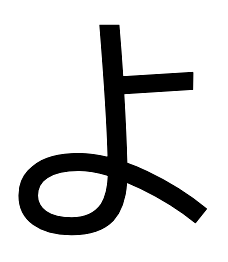
\includegraphics[width=0.27cm,height=0.27cm]{yon.png}$}
\newunicodechar{⊥}{$\bot$}
\newunicodechar{∼}{$\sim$}
\newunicodechar{≃}{$\simeq$}
\newunicodechar{≅}{$\cong$}
\newunicodechar{∞}{$\infty$}

\newunicodechar{α}{$\alpha$}
\newunicodechar{β}{$\beta$}
\newunicodechar{γ}{$\gamma$}
\newunicodechar{δ}{$\delta$}
\newunicodechar{ε}{$\epsilon$}
\newunicodechar{η}{$\eta$}
\newunicodechar{ζ}{$\zeta$}
\newunicodechar{θ}{$\theta$}
\newunicodechar{ι}{$\iota$}
\newunicodechar{μ}{$\mu$}
\newunicodechar{κ}{$\kappa$}
\newunicodechar{λ}{$\lambda$}
\newunicodechar{ρ}{$\rho$}
\newunicodechar{π}{$\pi$}
\newunicodechar{σ}{$\sigma$}
\newunicodechar{τ}{$\tau$}
\newunicodechar{υ}{$\upsilon$}
\newunicodechar{φ}{$\phi$}
\newunicodechar{ψ}{$\psi$}
\newunicodechar{ξ}{$\xi$}
\newunicodechar{χ}{$\chi$}
\newunicodechar{ω}{$\omega$}

\newunicodechar{⊗}{$\otimes$}

\makeatletter
\newcommand*{\shifttext}[2]{\settowidth{\@tempdima}{#2}\makebox[\@tempdima]{\hspace*{#1}#2}}
\makeatother
\definecolor{Red}{cmyk}{0.1, 0.70, 0.65, 0.00, 1.00}
\definecolor{Blue}{cmyk}{0.9, 0.2, 0.2, 0.00, 1.00}
\definecolor{Yellow}{cmyk}{0.0, 0.00, 0.7, 0.00, 0.5}
\definecolor{Green}{cmyk}{0.6, 0.0, 0.6, 0.00, 1.00}
\definecolor{Purple}{cmyk}{0.8, 0.3, 0.3, 0.00, 1.00}
\definecolor{Orange}{cmyk}{0.0, 0.3, 0.7, 0.00, 1.00}
\definecolor{Grey}{cmyk}{0.13, 0.13, 0.13, 0.00, 1.00}
\newcounter{definitioncounter}
\setcounter{definitioncounter}{1}
\newcounter{theoremcounter}
\setcounter{theoremcounter}{1}
\newcounter{printcounter}
\setcounter{printcounter}{1}
\newcounter{examplecounter}
\setcounter{examplecounter}{1}
\newcounter{ccounter}
\setcounter{ccounter}{1}
\newcounter{pcounter}
\setcounter{pcounter}{1}
\newcounter{lcounter}
\setcounter{lcounter}{1}
\newcounter{sectioncount}
\newcounter{subsectioncount}
\setcounter{sectioncount}{1}
\renewcommand{\section}[1]{\newpage\ \\ \ \\ \begin{center} \scalebox{1.5}{\texttt{\thesectioncount . #1}} \stepcounter{sectioncount} \setcounter{subsectioncount}{1} \end{center} \begin{center} \ \\ \ \\ \thispagestyle{empty} \end{center}}
\renewcommand{\subsection}[1]{\texttt{\thesubsectioncount . #1} \stepcounter{subsectioncount}}
\renewcommand{\backslash}{\reflectbox{\texttt{/}}}

\newcounter{chaptercount}
\renewcommand{\chapter}[1]{
\newpage
{
\Huge 
\begin{center}
\ \\
\ \\
\thispagestyle{empty}
\texttt{#1}
\end{center}}
\ \\
\ \\
}

\newcounter{partcount}
\stepcounter{partcount}
\renewcommand{\part}[1]{
\newpage
{
\Huge 
\begin{center}
\ \\
\ \\
\ \\
\ \\
\ \\
\ \\
\thispagestyle{empty}
\texttt{PART {\thepartcount}: #1}
\stepcounter{partcount}
\end{center}}
\ \\
\ \\
}


\begin{document}

\thispagestyle{empty} 

\AddToShipoutPicture*
    {\put(540,720){

    \href{http://www.linearlibrary.net}{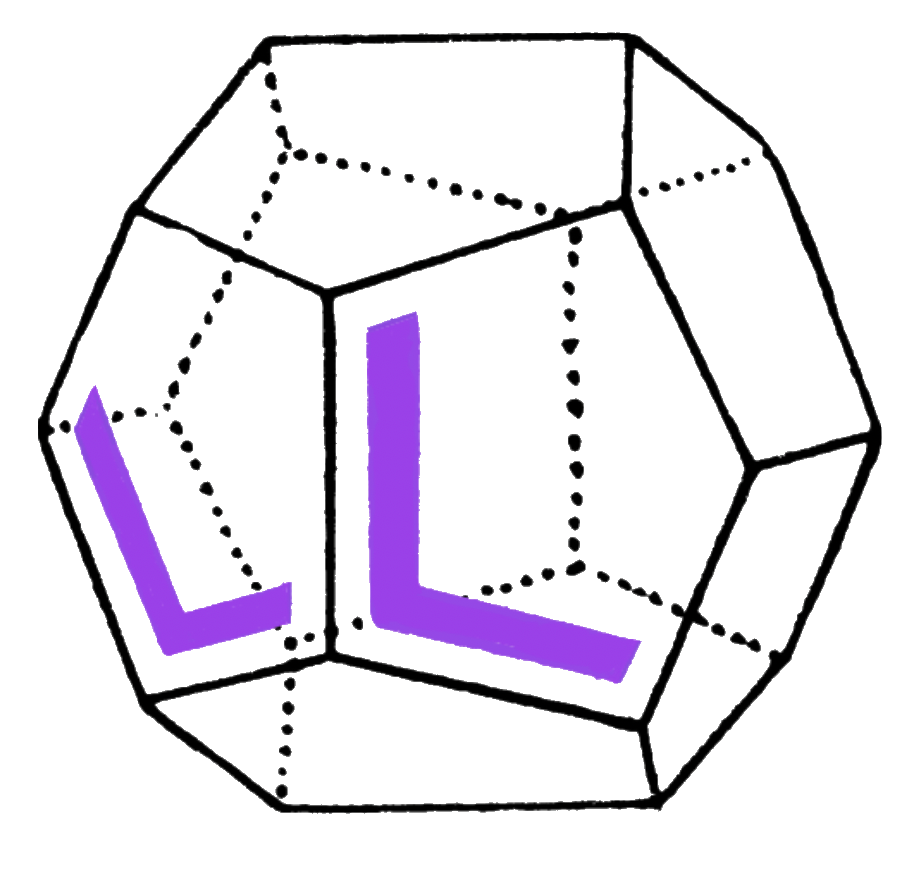
\includegraphics[width=2cm,height=2cm]{ll.png}}

    }}

\AddToShipoutPicture*
  {\put(470,767){
    \href{https://www.github.com/linlib/InfinitySpaces/blob/main/StringDiagramGenerator.py}{\texttt{.py file}}
  }}

\AddToShipoutPicture*
  {\put(470,752){
    \href{https://www.github.com/linlib/InfinitySpaces/blob/main/InfinitySpaces.tex}{\texttt{.tex file}}\\

  }}

\AddToShipoutPicture*
  {\put(470,737){

    \href{http://www.github.com/InfinitySpaces/blob/main/InfinitySpaces.pdf}{\texttt{.pdf file}}\\

  }}

  \AddToShipoutPicture*
  {\put(470,722){
    \href{https://www.github.com/linlib/InfinitySpaces/blob/main/InfinitySpaces.lean}{\texttt{.lean file}}

  }}

\ \\

%LEAN: 
\begin{center}
\begin{tcolorbox}[width=2.3in,colback={white},coltitle=white]
\begin{center}
\ \\
\scalebox{3}{\texttt{∞-Spaces}}\\
\end{center}
\end{tcolorbox}
\end{center}
\ \\
\ \\
\ \\
\begin{center}
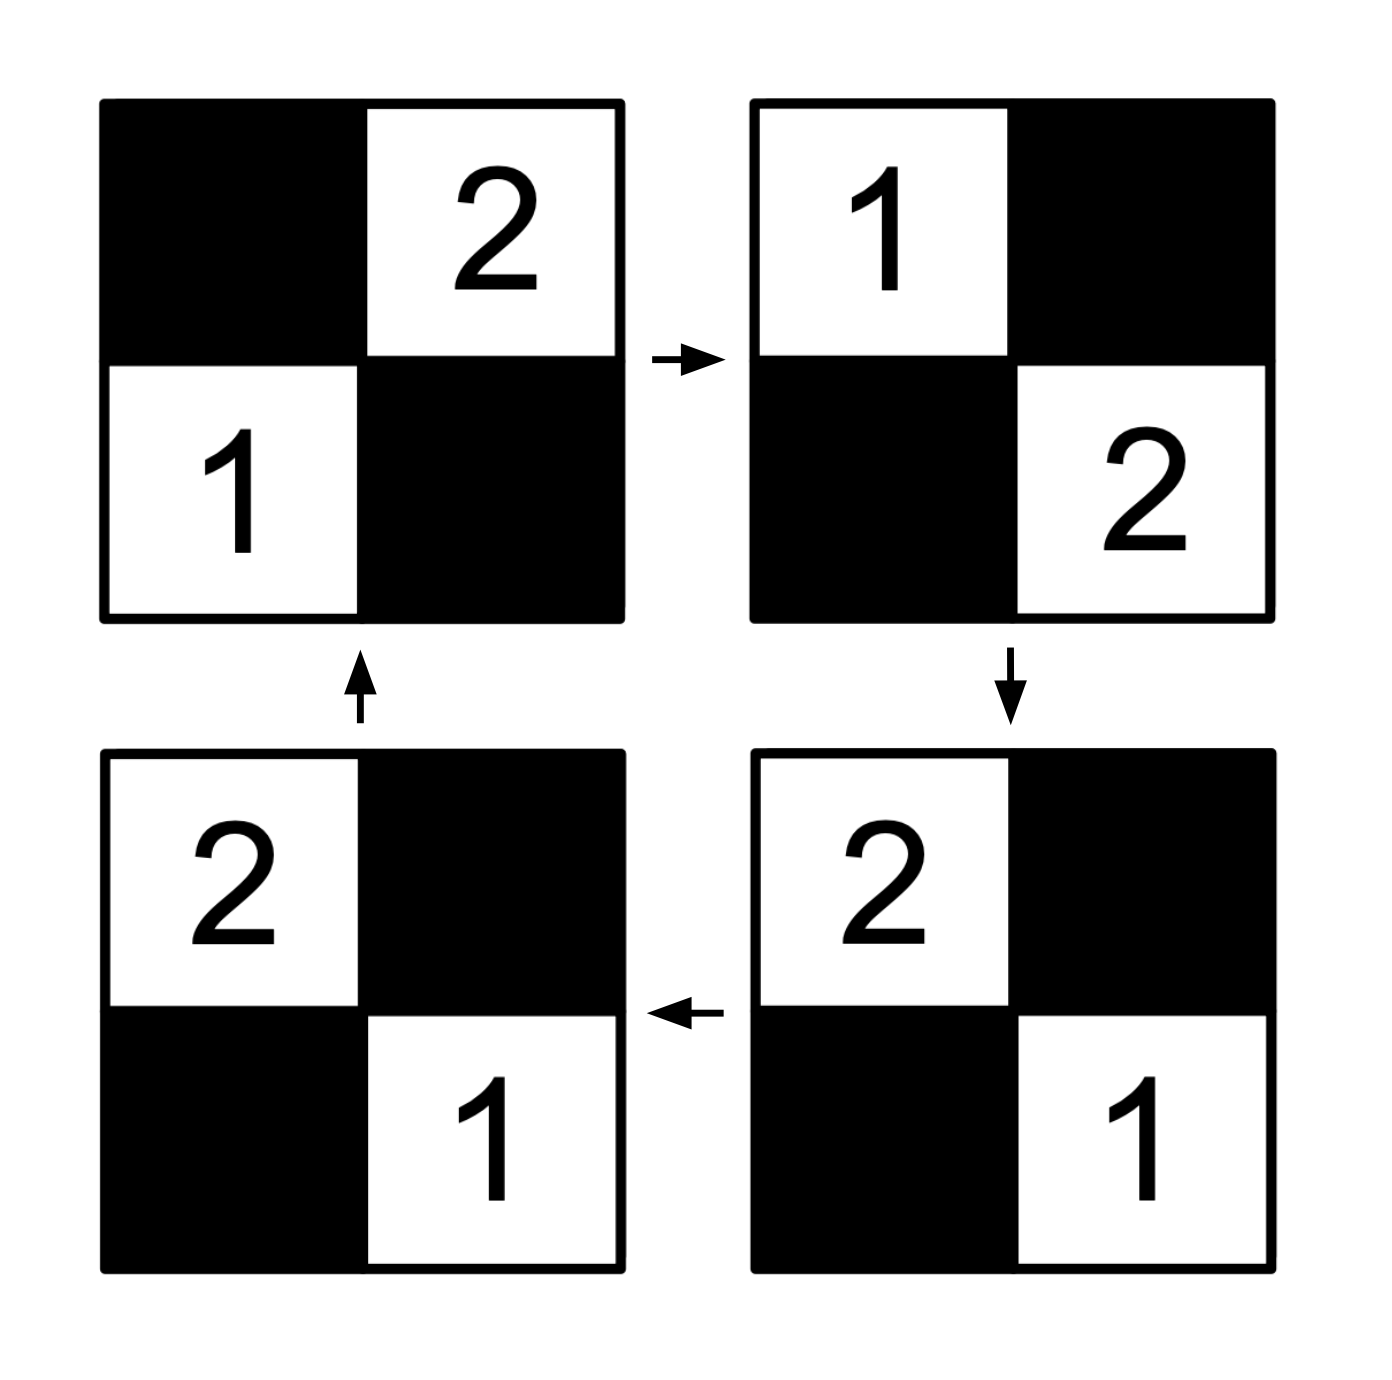
\includegraphics[scale=0.4]{eckhil.png}
\end{center}





\thispagestyle{empty}


\newpage


\begin{center}

\pagecolor{white}
\color{black}

\end{center}

\thispagestyle{empty}




\newpage
\pagecolor{white}
\color{black}
\ \\
\ \\
\thispagestyle{empty}

\large %%%%%%%% HERE IS THE large LARGE size textsize set text size
\newpage 
\ \\
\ \\
\ \\
\ \\
\ \\
\ \\
\ \\
\ \\
\ \\
\ \\
\ \\
\thispagestyle{empty}
 
\newpage

\ \\
\ \\
\ \\
\ \\
\ \\
\ \\
\ \\
\ \\
\ \\
\ \\
\ \\

\newpage


\iffalse
░▒▓█▓▒░░▒▓█▓▒░▒▓███████▓▒░░▒▓█▓▒░░▒▓██████▓▒░ ░▒▓██████▓▒░░▒▓███████▓▒░░▒▓████████▓▒░ 
░▒▓█▓▒░░▒▓█▓▒░▒▓█▓▒░░▒▓█▓▒░▒▓█▓▒░▒▓█▓▒░░▒▓█▓▒░▒▓█▓▒░░▒▓█▓▒░▒▓█▓▒░░▒▓█▓▒░▒▓█▓▒░        
░▒▓█▓▒░░▒▓█▓▒░▒▓█▓▒░░▒▓█▓▒░▒▓█▓▒░▒▓█▓▒░      ░▒▓█▓▒░░▒▓█▓▒░▒▓█▓▒░░▒▓█▓▒░▒▓█▓▒░        
░▒▓█▓▒░░▒▓█▓▒░▒▓█▓▒░░▒▓█▓▒░▒▓█▓▒░▒▓█▓▒░      ░▒▓█▓▒░░▒▓█▓▒░▒▓█▓▒░░▒▓█▓▒░▒▓██████▓▒░   
░▒▓█▓▒░░▒▓█▓▒░▒▓█▓▒░░▒▓█▓▒░▒▓█▓▒░▒▓█▓▒░      ░▒▓█▓▒░░▒▓█▓▒░▒▓█▓▒░░▒▓█▓▒░▒▓█▓▒░        
░▒▓█▓▒░░▒▓█▓▒░▒▓█▓▒░░▒▓█▓▒░▒▓█▓▒░▒▓█▓▒░░▒▓█▓▒░▒▓█▓▒░░▒▓█▓▒░▒▓█▓▒░░▒▓█▓▒░▒▓█▓▒░        
 ░▒▓██████▓▒░░▒▓█▓▒░░▒▓█▓▒░▒▓█▓▒░░▒▓██████▓▒░ ░▒▓██████▓▒░░▒▓███████▓▒░░▒▓████████▓▒░
\fi
\newpage
\section{Unicode}

Here is a list of the unicode characters we will use:

{\footnotesize
\begin{center}
\begin{tabular}{|| l || l || l || l ||} 
\hline
$\texttt{Symbol}$ & $\texttt{Unicode}$ & \texttt{VSCode shortcut} & $\texttt{Use}$\\
\hline
\hline
\multicolumn{4}{||c||}{\texttt{Lean's Kernel}} \\
\hline
\hline
× & 2A2F & \backslash\texttt{times} & Product of types\\
\hline
→ & 2192 & \backslash\texttt{rightarrow}  & Hom of types\\
\hline
⟨,⟩ & 27E8,27E9 & \backslash\texttt{langle},\backslash\texttt{rangle}  & Product term introduction\\
\hline
↦ & 21A6 &\backslash\texttt{mapsto}  & Hom term introduction\\
\hline
∧ & 2227 &\backslash\texttt{wedge}  & Conjunction \\
\hline
∨ & 2228 &\backslash\texttt{vee}  & Disjunction \\
\hline
∀ & 2200 &\backslash\texttt{forall}  & Universal quantification \\
\hline
∃ & 2203 &\backslash\texttt{exists}  & Existential quantification\\
\hline
¬ & 00AC &\backslash\texttt{neg}  & Negation\\
\hline
\hline
\multicolumn{4}{||c||}{\texttt{Variables and Constants}} \\
\hline
\hline
ᵃ,ᵇ,ᶜ,...,ᶻ & 1D52,1D56 & & Variables and constants \\
\hline
⁰,¹,²,³,⁴,⁵,⁶,⁷,⁸,⁹ & 1D52,1D56 &  & Variables and constants \\
\hline
⁻ & 207B &  & Variables and constants \\
\hline
₀,₁,₂,₃,₄,₅,₆,₇,₈,₉ & 2080 - 2089 & \backslash\texttt{0}-\backslash\texttt{9} & Variables and constants\\
\hline
𝔸,...,ℤ & 1D538 &  &  \\
\hline
𝕒,...,𝕫 & 1D552 &  &  \\
\hline
𝐀,...,𝐙 & 1D41A &  &  \\
\hline
𝐚,...,𝐳 & 1D41A &  &  \\
\hline
\texttt{α}-\texttt{ω},\texttt{A}-\texttt{Ω} & 03B1-03C9 & & Variables and constants\\
\hline
\hline
\multicolumn{4}{||c||}{\texttt{Categories}} \\
\hline
\hline
 𝟙 & 1D7D9 & \backslash\texttt{b1}  & The identity morphism\\
\hline
 ∘ & 2218 & \backslash\texttt{circ}  & Composition\\
 \hline
 \hline
 \multicolumn{4}{||c||}{\texttt{Bicategories}} \\
 \hline 
 \hline
 • & 2022  & \backslash\texttt{smul}  & Horizontal composition of objects\\ 
  \hline
  \hline
 \multicolumn{4}{||c||}{\texttt{Adjunctions}} \\
\hline
\hline
⇄ & 21C4 & \backslash\texttt{rightleftarrows}  & Adjunctions \\
\hline
⇆ & 21C6 & \backslash\texttt{leftrightarrows}  & Adjunctions \\
\hline
𛲔 & 1BC94 &  & Right adjoints\\
\hline
ॱ & 0971 &  & Left adjoints \\
\hline
⊣ & 22A3 & \backslash\texttt{dashv}  & The condition that two functors are adjoint \\
\hline
\hline
\multicolumn{4}{||c||}{\texttt{Monads and Comonads}} \\
\hline
\hline
?,¿ & 003F, 00BF & ?,\backslash\texttt{?}  & The corresponding (co)monad of an adjunction\\
\hline
!,¡ & 0021, 00A1 & !, \backslash\texttt{!}  & The (co)-Eilenberg-(co)-Moore adjunction \\
\hline
ꜝ,ꜞ & A71D, A71E &  & The (co)exponential maps\\
\hline
\hline
\multicolumn{4}{||c||}{\texttt{Miscellaneous}} \\
\hline
\hline
∼ & 223C & \backslash\texttt{sim} & Homotopies \\
\hline
≃ & 2243 & \backslash\texttt{equiv}  & Equivalences \\
\hline
≅ & 2245 & \backslash\texttt{cong}  & Isomorphisms \\
\hline
⊥ & 22A5 & \backslash\texttt{bot}  & The overobject classifier \\
\hline
∞ & 221E & \backslash\texttt{infty}  & Infinity categories and infinity groupoids\\ 
\hline
${}^{\leftrightarrow}$ & 20D7 &  & Homotopical operations on ∞-categories \\
\hline
${}^{\rightarrow}$ & 20E1 &  & Homotopical operations on ∞-groupoids \\
\hline
\end{tabular}
\end{center}}

\section{Introduction}

\noindent\textcolor{Red}{\rule{16cm}{1mm}}
\begin{center}
\texttt{Implementation Progress}
\end{center}
\noindent\textcolor{Red}{\rule{16cm}{1mm}}

\noindent\textcolor{Red}{\rule{16cm}{1mm}}
\begin{center}
\texttt{Writing Progress}
\end{center}
\noindent\textcolor{Red}{\rule{16cm}{1mm}}

How d is to D as unitial is to actional, and yet d² is 0 for chain complexes (different than globular sets), and not so for D. This suggests that we consider complexes in general rather than those particular complexes arising from globular abelian groups or globular ∞-spaces, in which d² = 0. What remains is an understanding of tensor product and a "sign" which accompanies it. Even though tensor product is determined up to isomorphism by being adjoint to a graded hom, the addition of the sign allows for the free DGA and free differential graded ∞-space constructions.\\

Hence in this document we take the approach of thinking about presheaves and ∞-presheaves over the diagram ⋯ ⭢ • ⭢ • ⭢ • ⭢ ⋯, without a square-zero condition. Those presheaves (in abelian groups) and ∞-presheaves (in ∞-spaces) which arise from ∞-groupoids have this condition, but reside within a larger situation in which the main constructions extend.\\

All of this produces less confusion in regards to \\


Eℕ...\\



\begin{enumerate}
\item A functorial construction of the classifying space in homotopy which can be applied indefinitely.
\item This construction will be an endofunctor of operadic groups in operadic groups in ∞-Grpd.
\item I would like to notate it as B¹. 
\end{enumerate}

The topics here feature the Eckman-Hilton argument and the abelian nature of π₂ at their core. We can understand these using continuous functions out of the square of the unit interval γ⃡² or the square of the directed unit interval γ⃗². In the case of a based ∞-groupoid X, π₂ is first defined using continuous functions f : I² ⭢ X such that f((x,y)) is sent to the base of X when either x or y is 0.\\

This notation distinguishes 

my attempt at an abelian-classifying-space construction which is an endofunctor of grouplike E${}^{\infty}$-spaces, here refered to as ∞-spaces, from the classifying-space construction involving ∞-groupoids and grouplike A${}^{\infty}$-spaces. Note that our ∞-categories always have r = 1, i.e. ∞ is short for (∞,1).\\

I will write Bⁿ for the n-fold composition of B¹, Pow B n. Note that B is not an endofunctor so that it cannot be iterated. It is more typical to divide up the construction B, for instance constructing the Grassmanians Gr${}^{\infty}$(ℂ,n) ≅ B.obj GLₙ(ℂ), from which it follows that [-,Gr${}^{\infty}$(ℂ,n)] is equivalent to the category of GLₙ(ℂ)-principal bundles and therefore to n-dimensional vector bundles bundles.\\

In ```TheWhiteheadTheoremandTwoVariations''', we developed two models of ∞-Grpd\_(A) and ∞-Grpd\_(B). These will produce two models on which B¹ can be defined:

\begin{center}
B¹ : OperadicGroup • OperadicGroup ∞-Grpd ⭢ OperadicGroup • OperadicGroup ∞-Grpd
\end{center}

\iffalse
Without compactness or local compactness we only have an operadic smash product.
\fi

\iffalse
The category of ∞-spaces intermediates the category of spectra and the category of ∞-groupoids.\\
\fi

\iffalse
https://www.youtube.com/watch?v=I81DHkDNfTs
\fi

\iffalse
The natural and organic failures that have come before make people apprehensive about the straightforward approach here.
\fi


\iffalse
https://redprl.org/
agda
rzk (new!)
\fi

\iffalse
- glueing in with Joel Riou's API (powerful)
- convenient widgets
\fi


\iffalse
https://mathoverflow.net/questions/464176/bⁿ-and-coherence
\fi

after this we develop chain complexes of these.\\

The table of contents below reflects the tentative long-term goals of the authors, with the main goal the pursuit of the Whitehead theorem for a point-set model involving Mathlib's predefined homotopy groups.\\

\begin{enumerate}
\item cup and cap product
\end{enumerate}

Ideas for future applications:

\begin{enumerate}
\item \url{https://arxiv.org/pdf/2206.13563.pdf}
\end{enumerate}

\begin{enumerate}
\item One of the basic things I wanted out of this was homotopy colimit preserving maps (Eⁱⁿᶠ-Alg A)ᵒᵖ ⭢ ∞-Grpd
\end{enumerate}

Note that this repository does not implement $\texttt{Q X := colimitₙ Ωⁿ Σⁿ X}$ or the stable homotopy groups. It concerns the relationship between O and B and not Ω and Σ.\\

\iffalse
A famous paper of ... demonstrates the inconsistency of five conditions related to Ωⁱⁿᶠ : ∞-Grpd₋₁ ⇄ Spectra : Σⁱⁿᶠ. This problem is here solved by adding in the intermediate category of ∞-spaces:

∞-Grpd₋₁ ⇄ ∞-Space ⇄ Spectra

Meanwhile the tensor product of chain complexes is 

The first of these adjunctions is the free abelian group construction whose counit is associated to a version of the Dold-Thom theorem.\\

The second of these adjunctions is the `true` infinite delooping and infinite looping, featuring an analogue of all five theorems. Given the intermediate construction of infinite loop spaces, it is possible to form Spectra as a higher inverse limit of ∞-Space in which Σ is invertible. The loop space in ∞-spaces is constructed so that 
\fi

\begin{enumerate}
\item Complexes of abelian groups and ∞-spaces are the same as ∞-presheaves on E.obj ℕ.
\item 
\end{enumerate}

\section{Contents}


{
\footnotesize
\begin{longtable}{|| l || l ||} 
\hline
\multicolumn{1}{||c||}{$\texttt{Section}$} & \multicolumn{1}{|c||}{$\texttt{Description}$} \\
\hline
\hline
Unfinished & \\
\hline
Contents & \\
\hline
Unicode & \\
\hline
Introduction & \\
\hline \hline
\multicolumn{2}{||c||}{\texttt{PART I: } ∞-SPACES} \\
\hline \hline
 \multicolumn{2}{||c||}{\texttt{Chapter 1: }Abelian Groups} \\
\hline \hline
abeliangroup & The type of abelian groups \\
\hline
Maps of abelian groups & Constructing homomorphisms of abelian groups \\
\hline
Negation & \\
\hline
The Eckman-Hilton Argument & \\
\hline
AbelianGroup ⭢ Group & The forgetful functor from abelian groups to groups \\
\hline
Eilenberg-Maclane Spaces & \\
\hline
Chain Complexes & \\
\hline
Realization of Chain Complexes & \\
\hline
Tensor Product of Chain Complexes & \\
\hline \hline
 \multicolumn{2}{||c||}{\texttt{Chapter 2: }∞-Spaces} \\
\hline \hline
∞-space & The type of ∞-spaces \\
\hline
Maps of ∞-spaces & Constructing maps of ∞-spaces \\
\hline
Negation & \\
\hline
The Eckman-Hilton Argument & \\
\hline
OperadicGroup OperadicGroup ∞-Grpd₋₁ ⭢ OperadicGroup ∞-Grpd₋₁ & \\
\hline
B¹ and Bⁿ & \\
\hline
Chn : ??? & \\
\hline
Realization of Chain Complexes & \\
\hline
Tensor Product of Chain Complexes & \\
\hline \hline
\multicolumn{2}{||c||}{\texttt{Chapter 3: }Tensor Product of Abelian Groups} \\
\hline \hline
- ⊗\_(AbelianGroups) - & Mathlib's tensor product of abelian groups \\
\hline
[-,-]\_(AbelianGroups) & Mathlib's hom of abelian groups\\
\hline
AbelianGroup & The symmetric monoidal category of abelian groups\\
\hline \hline
\multicolumn{2}{||c||}{\texttt{Chapter 4: }Tensor Product of ∞-Spaces} \\
\hline \hline
- ⊗\_(∞-Space) - &  \\
\hline
[-,-]\_(∞-Space) &  \\
\hline
∞-Space & The symmetric monoidal category of ∞-spaces \\
\hline \hline
 \multicolumn{2}{||c||}{\texttt{Chapter 5: }Set₋₁ ⇄ AbelianGroups} \\
\hline \hline
??? & The free abelian group functor \\
 \hline
??? & The forgetful functor from abelian groups to pointed sets \\
 \hline
??? : Set₋₁ ⇄ AbelianGroup : ??? & The adjunction between pointed sets and abelian groups \\
\hline \hline
 \multicolumn{2}{||c||}{\texttt{Chapter 6: }∞-Grpd₋₁ ⇄ ∞-Space} \\
\hline \hline
??? & The free ∞-space given a based ∞-groupoid \\
\hline
??? & The forgetul functor from ∞-spaces to ∞-groupoids \\
\hline
??? : ∞-Grpd₋₁ ⇄ ∞-Space : ??? & The ??? between ∞-Grpd₋₁ and ∞-Spaces \\
\hline \hline
\multicolumn{2}{||c||}{\texttt{PART II: } RINGS, COMMUTATIVE RINGS, A${}^{\infty}$-RINGS, AND E${}^{\infty}$-RINGS} \\
\hline \hline
\multicolumn{2}{||c||}{\texttt{Chapter 7: }Rings and Commutative Rings} \\
\hline \hline
ring & The type of rings \\
 \hline
Ring & The category of rings \\
\hline
commutative\_ring & The type of commutative rings  \\
\hline
CommutativeRing & The category of commutative rings \\
 \hline \hline
  \multicolumn{2}{||c||}{\texttt{Chapter 8: }A${}^{\infty}$-Rings and E${}^{\infty}$-Rings} \\
\hline \hline
A${}^{\infty}$-ring & The type of A${}^{\infty}$-rings \\
\hline
A${}^{\infty}$-Ring & The category of A${}^{\infty}$-Rings \\
 \hline
E${}^{\infty}$-ring  & The type of E${}^{\infty}$-rings \\
 \hline
E${}^{\infty}$-Ring  & The category of E${}^{\infty}$-Rings \\
 \hline \hline
\multicolumn{2}{||c||}{\texttt{Chapter 9: }Modules and Modules over Commutative Rings} \\
\hline \hline
 &  \\
 \hline
 &  \\
 \hline
InternalMonoidAction (InternalMonoid C) ≅ InternalMonoid (InteralMonoidAction C) & The ??? theorem \\ 
\hline
CommutativeAlgebra : CommutativeRing → Cat & The category of commutative algebras \\
\hline
Maps (Algebra A) : Cat & The category of maps of commutative A-algebras \\
\hline \hline
\multicolumn{2}{||c||}{\texttt{Chapter 10: }A${}^{\infty}$-Modules and E${}^{\infty}$-Modules} \\
\hline \hline
 &  \\
\hline
 &  \\
\hline
$A{}^{\infty}$-RingAction ($A{}^{\infty}$-Ring C) ≅ $A{}^{\infty}$-Ring ($A{}^{\infty}$-RingAction C) & The ??? theorem \\ 
\hline
Maps A${}^{\infty}$-Algebras & \\
 \hline \hline
\multicolumn{2}{||c||}{\texttt{PART III: } DERIVATIONS AND CONNECTIONS} \\
\hline \hline
\multicolumn{2}{||c||}{\texttt{Chapter 11: }Lie Algebras} \\
\hline \hline
lie\_algebra & The type of Lie-algebras \\
\hline
LieAlgebra & The category of Lie-algebras \\
\hline \hline
\multicolumn{2}{||c||}{\texttt{Chapter 12: }Derivations} \\
\hline \hline
InternalAbelianGroup (Maps (Algebra A)) ≅ MonoidActionObject A & ??? \\
\hline
??? : (Maps (Algebra A)) ⇄ InternalAbelianGroup (Maps (Algebra A)) : ??? & The free abelian group functor for (Maps (Algebra A)) \\
\hline
Λ : ??? ⇄ ??? : FstDeg & \\ 
\hline
??? : (Algebra A) ⇄ Chn (Algebra A) : ??? & The free DGA functor \\
\hline 
derivation & Definition of a derivation \\
\hline
Der : () ⇄ (InternalMonoidAction A) : ??? & A derivation is a primitive element \\
\hline \hline
\multicolumn{2}{||c||}{\texttt{Chapter 13: }L${}^{\infty}$ Algebras} \\
\hline \hline
Lⁱⁿᶠ\_algebra & The type of L${}^{\infty}$-algebras  \\
\hline
L${}^{\infty}$Algebra &  \\
\hline \hline
\multicolumn{2}{||c||}{\texttt{Chapter 14: }∞-Derivations} \\
\hline \hline
OperadicAbelianGroup (Maps (∞-Algebra A)) ≅ E${}^{\infty}$-MonoidAction A & ??? \\
\hline
??? : $A{}^{\infty}$-Algebras ⇄ ???  & The free abelian group \\
\hline
Λ : ??? ⇄ ??? : FstDeg &  \\ 
\hline
??? : (???) ⇄ (???) : ??? & The free ??? \\
\hline
∞-derivation & Definition of an ∞-derivation \\
\hline
∞-Der : () ⇄ () : ??? & A derivation is an ∞-primitive element \\
\hline \hline
\multicolumn{2}{||c||}{\texttt{Chapter 15: }Tensor Product of Lie Algebras} \\
\hline \hline
- ⊗\_() - &  \\
\hline
LieAlgebra : ??? & The monoidal category of Lie algebras\\
\hline \hline
\multicolumn{2}{||c||}{\texttt{Chapter 16: }Tensor Product of L${}^{\infty}$-Algebras} \\
\hline \hline
- ⊗\_() - & \\ 
 \hline
 : ??? & The symmetric monoidal category of L${}^{\infty}$-algebras \\
 \hline \hline
\multicolumn{2}{||c||}{\texttt{Chapter 17: }Lie Algebra Representations} \\
\hline \hline
 & \\
\hline
 & \\
\hline \hline
\multicolumn{2}{||c||}{\texttt{Chapter 18: }Connections} \\
\hline \hline
??? & The ??? equivalence \\
\hline
??? & The free internal abelian group action functor \\
\hline
??? & The first degree of the free E${}^{\infty}$-DGM on an algebra is s\_() \\
\hline
???   & ??? \\
\hline
connection & Definition of a connection \\
\hline
??? & A connection is a d-action \\
\hline \hline
\multicolumn{2}{||c||}{\texttt{Chapter 19: }L${}^{\infty}$-Representations} \\
\hline \hline
 & \\
\hline
 & \\
\hline \hline
\multicolumn{2}{||c||}{\texttt{Chapter 20: }∞-Connections} \\
\hline \hline
??? & The ??? equivalence \\
\hline
??? & The free operadic abelian group action functor \\
\hline
??? & The first degree of the free E${}^{\infty}$-DGM on an algebra is sⁱⁿᶠ\_() \\
\hline
???  & ??? \\
\hline
connection & Definition of a connection \\
\hline
??? & A connection is a dⁱⁿᶠ-action\\
\hline \hline
\multicolumn{2}{||c||}{\texttt{Chapter 21: }Tensor Product of Lie-Algebra Representations} \\
\hline \hline
- ⊗\_() - &  \\
\hline
[-,-]\_() &  \\
\hline
??? & The symmetric monoidal closed category of Lie-algebra representations \\
\hline \hline
\multicolumn{2}{||c||}{\texttt{Chapter 22: }Tensor Product of L${}^{\infty}$-Algebra Representations} \\
\hline \hline
- ⊗\_() -  &  \\
 \hline
[-,-]\_() - &  \\
 \hline
??? & The symmetric monoidal closed category of L${}^{\infty}$-algebra representations\\
 \hline \hline
\end{longtable}
}



\part{ABELIAN GROUPS AND ∞-SPACES}

In this first section I will construct eight structures for monoidal categories. These structures will be constructed so as to be endofunctions of a particular kind of monoidal category (as opposed to a cartesian category).\\


{
\footnotesize
\begin{center}
\begin{tabular}{||l || l || l || l ||} 
 \hline
  \multicolumn{4}{||c||}{\texttt{Eight Structures}} \\
 \hline
 \multicolumn{2}{||c||}{\texttt{Strict}}  &  \multicolumn{2}{||c||}{\texttt{Lax}} \\
 \hline
 \texttt{Unitial} &  \texttt{Actional}  &  \texttt{Unitial} &  \texttt{Actional}\\
 \hline \hline
 \texttt{InternalCommutativeMonoid} & \texttt{InternalCommutativeMonoidAction} & \texttt{OperadicCommutativeMonoid} & \texttt{OperadicCommutativeMonoidAction} \\
 \hline
 \texttt{InternalAbelianGroup} & \texttt{InternalAbelianGroupAction} & \texttt{OperadicAbelianGroup} & \texttt{OperadicAbelianGroupAction} \\
 \hline
\end{tabular}
\end{center}
}

One particular kind of monoidal category is a $\textit{cartesian category}$, i.e. a monoidal category in which the monoidal operation is cartesian product. Fox's theorem says that a symmetric monoidal category is cartesian if and only if it is isomorphic to cocommutative comonoids in itself. 

\iffalse
The repository concerning category at the linlib github will eventually feature a proof of this theorem..
\fi

We will also be interested to form the tensor product of abelian groups and the tensor product of ∞-spaces.

\iffalse
I will also construct internal abelian groups and a strcture I call `operadic abelian groups'.\\ 

One interesting object we will be able to construct is the tangent bundle on the unit ball in l₂(ℝ) and l₂(ℂ). 

Smooth functions on the unit ball in l₂ ...\\
\fi




\newpage
\chapter{Abelian Groups}

\section{The Category of Commutative Monoids and the Category of Abelian Groups}

\section{AbelianGroup ⭢ Group}

In this chapter I cover the type of abelian groups as well as the category of abelian groups.\\

\begin{enumerate}
\item Mathlib.Algebra.Group.Defs
\end{enumerate}




\iffalse
, CommutativeMonoid ⭢ Monoid
\fi


\section{Negation}




\section{The Eckman-Hilton Argument} 

The \href{https://ncatlab.org/nlab/show/Eckmann-Hilton+argument}{Eckman-Hilton Argument} demonstrates that internal groups in the monoidal category of groups with product as monoidal operation is equivalent to the category of abelian groups.\\



\section{Eilenberg-Maclane Spaces}

\begin{definition}
Let $\texttt{A}$ be an abelian group, and let $n \in \mathbb{N}$ be a non-negative integer. An Eilenberg-Maclane space .
\end{definition}


\subsection{The Postnikov Tower}


\subsection{The Whitehead Tower}


\section{Chain Complexes}

\begin{definition}
...
\end{definition}


\section{Realization of Chain Complexes}

\begin{definition}
...
\end{definition}


\section{Tensor Product of Chain Complexes}

\begin{definition}
...
\end{definition}

\iffalse
make sure to include commutative monoids
\fi


\newpage
\chapter{∞-Spaces}

\iffalse
Some choices of models for ∞-spaces are:
\begin{enumerate}
\item Algebras for the little discs operad
\item Algebras for the little squares operad in ∞-Cat
\item Algebras for the little lines operad in algebras for the little lines operad in ∞-Grpd
\item Algebras for the piecewise-linear-amortizations operad in algebras for the piecewise-linear-amortizations operad
\item Algebras for the 
\end{enumerate}
\fi

\section{The category of ∞-Spaces and the category of E${}^{\infty}$-Spaces}

\begin{center}
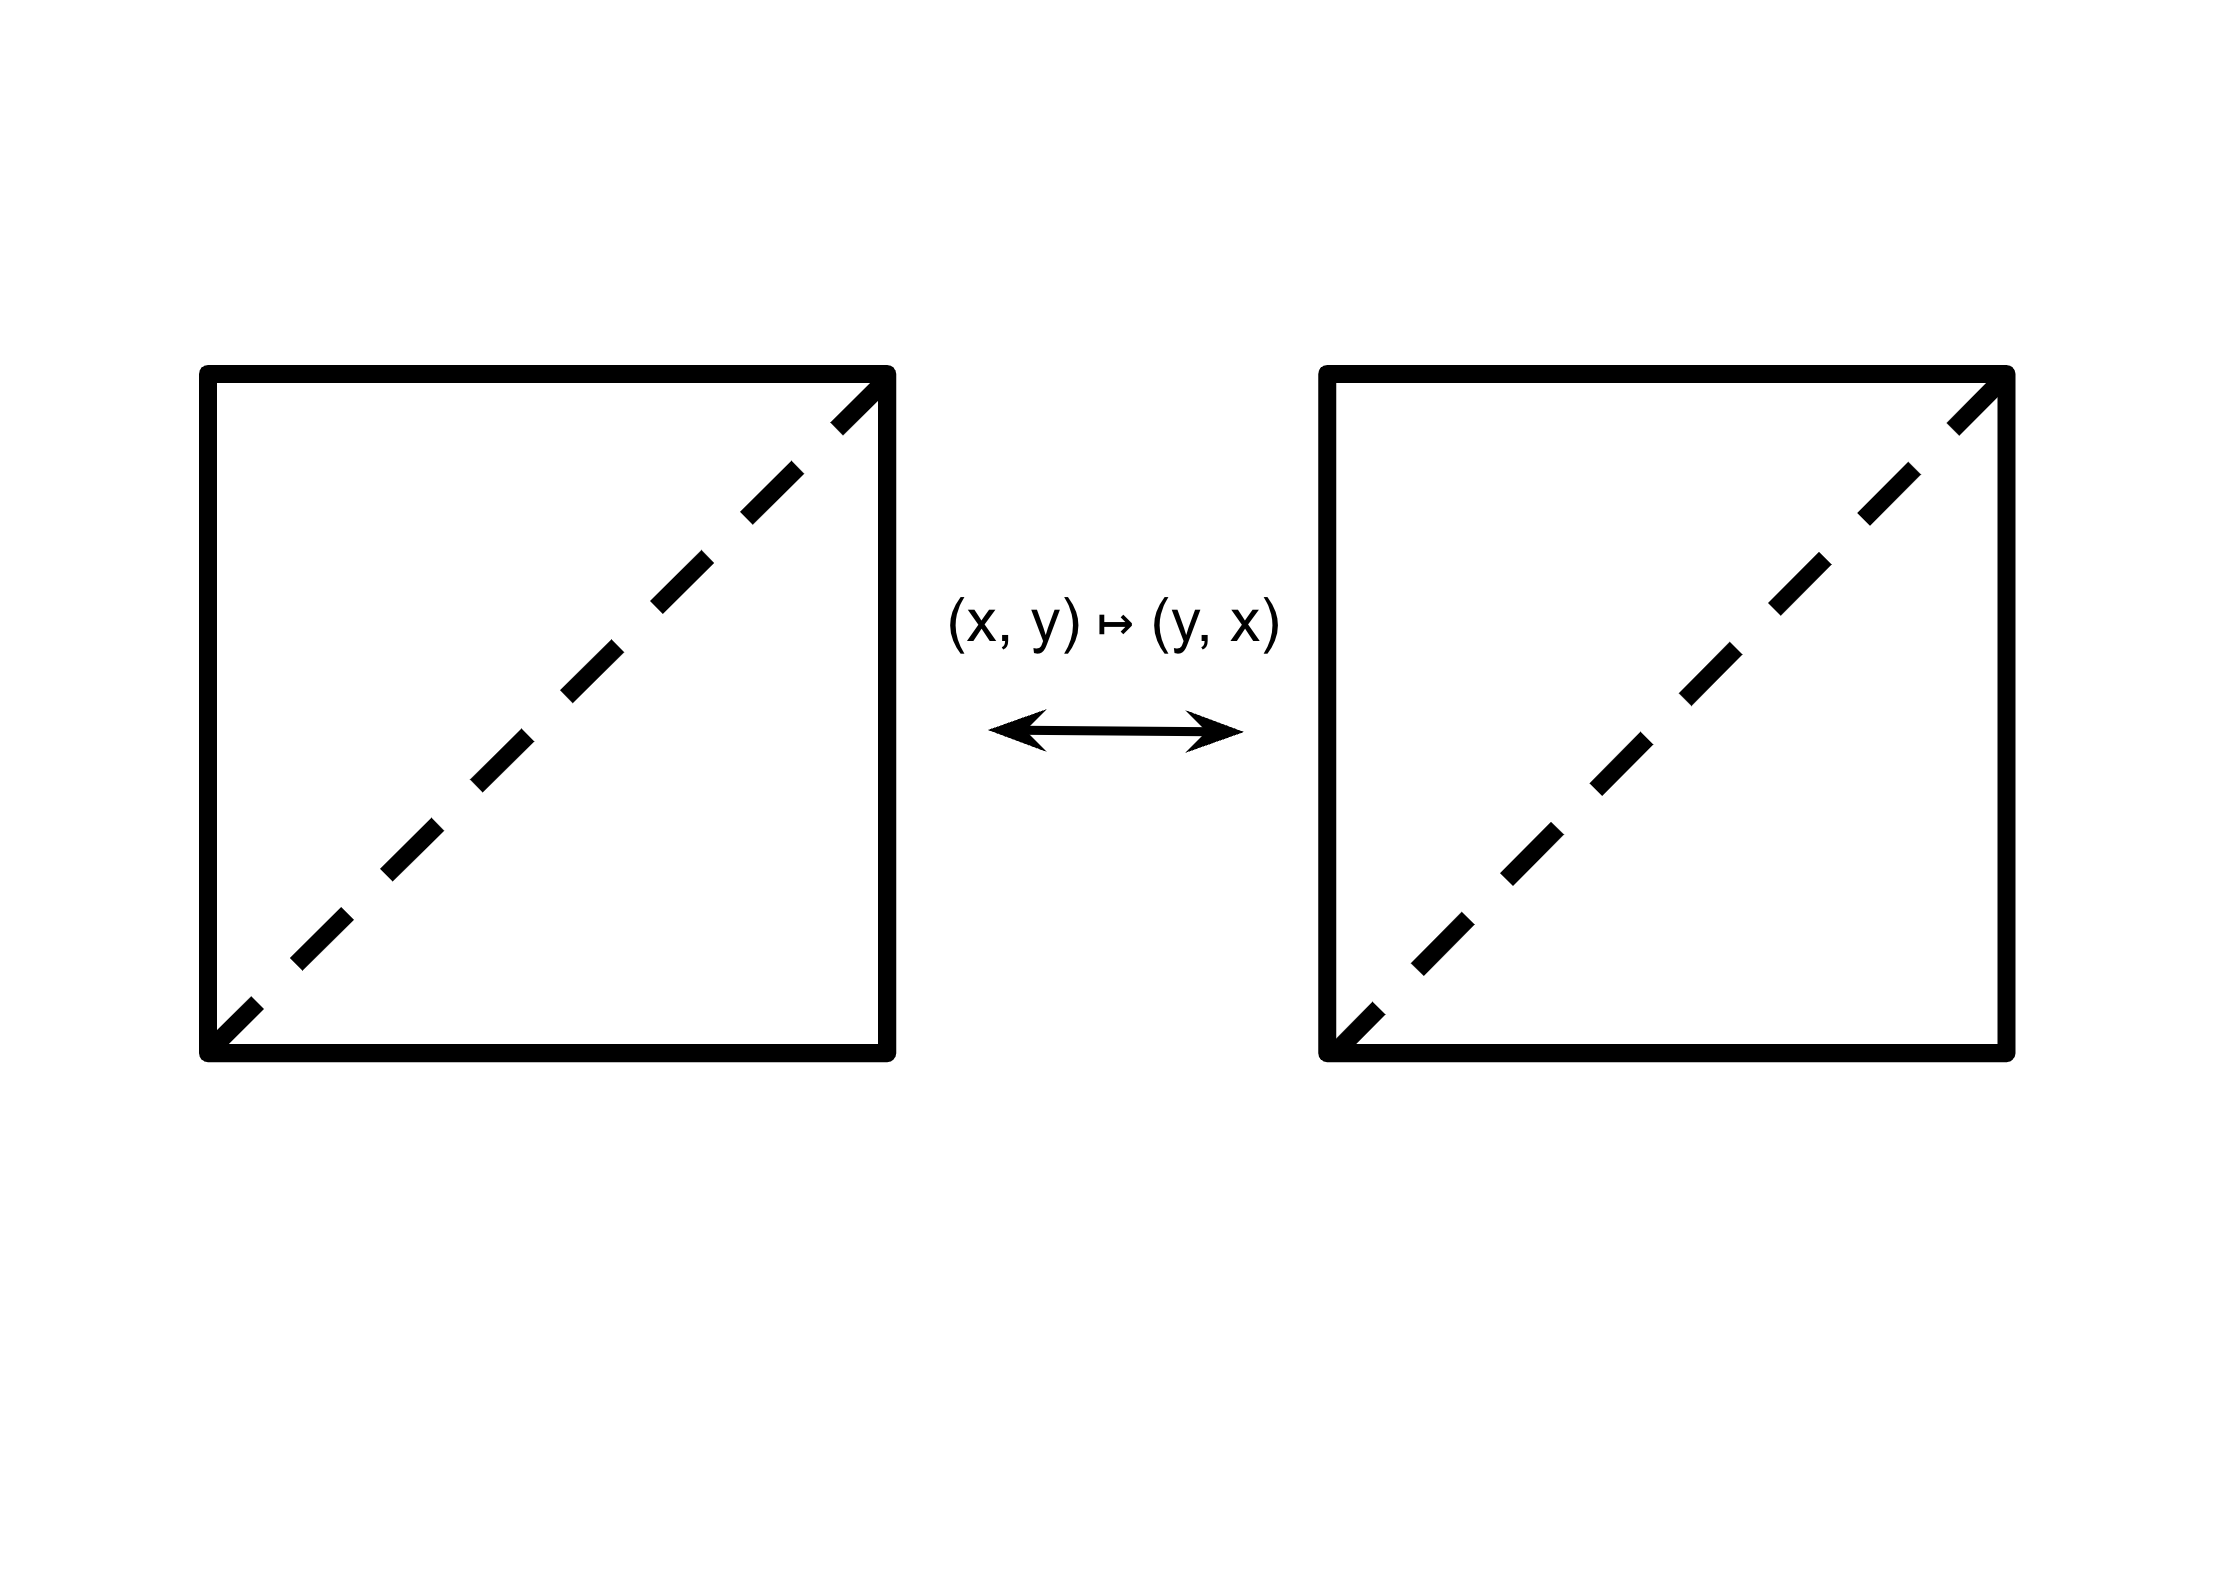
\includegraphics[scale=1]{littlesquaresA.png}
\end{center}

\begin{center}
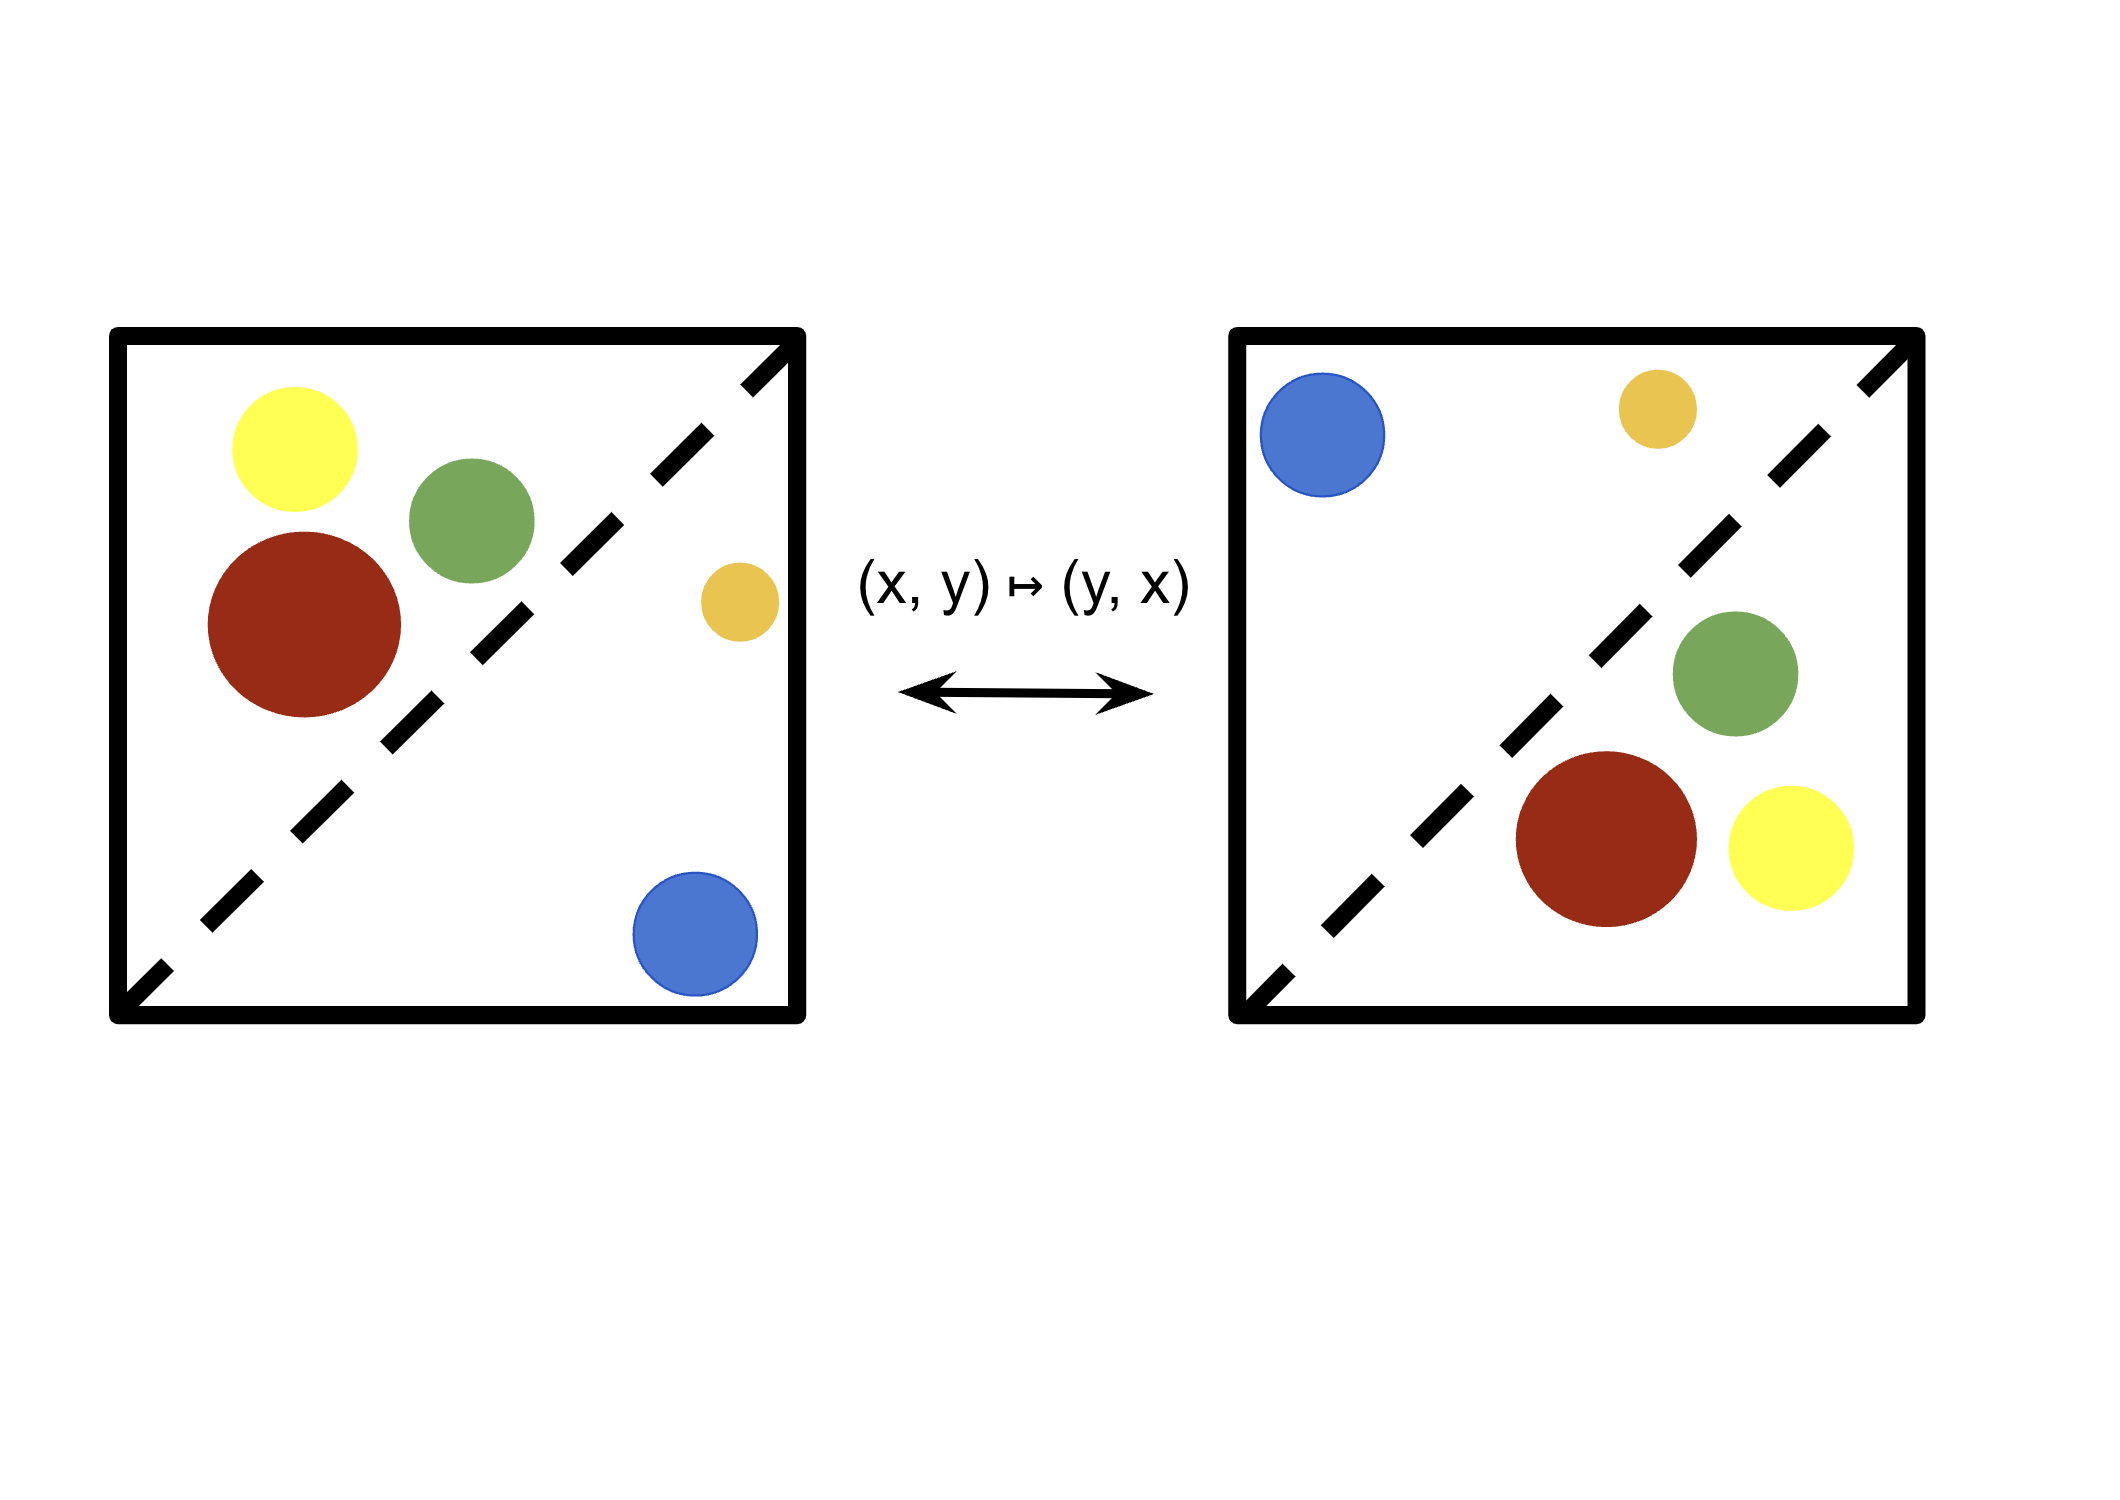
\includegraphics[scale=1]{littlesquaresB.png}
\end{center}


\section{∞-Spaces ⭢ OperadicGroup • OperadicGroup ∞-Grpd₋₁}

An ∞-space is an algebra for the little-squares operad.\\

The little-squares operad is OperadicGroup 2 ∞-Grpd.\\

, which we have here taken to mean an operadic group in operadic groups in based connected ∞-groupoids, is a particular operadic group. In this approach, we have considered OperadicGroup to have type ℕ ⭢ Cat rather than ∞-Cat ⭢ ∞-Cat or ∞\_(∞-Cat) ⭢ ∞\_(∞-Cat). Specifically, we can supply a non-negative integer to obtain a particular operad resembling little n-cubes but which features no "empty space".\\

\iffalse
, ∞⃗-Spaces ⭢ OperadicMonoid • OperadicMonoid ∞-Cat₋₁
\fi


\section{Negation}

For an ∞-space A, negation ¬ : A ⭢ A ...\\

∞-spaces


\section{The Eckman-Hilton Argument} 

\begin{center}
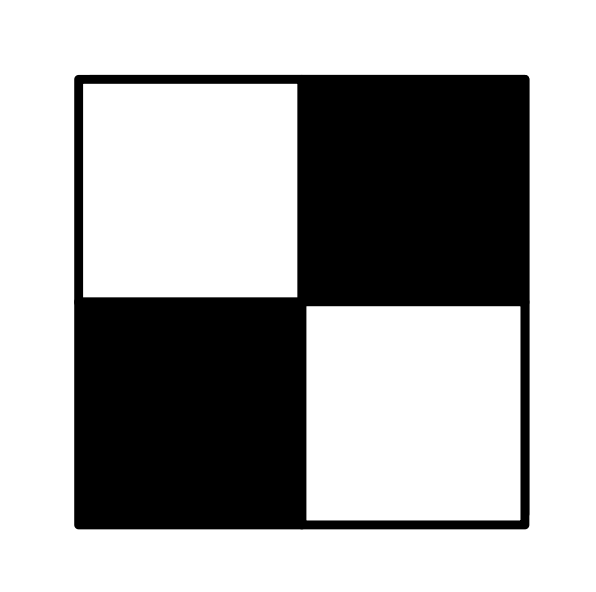
\includegraphics[scale=1]{eckmanhilton1.png}
\end{center}

\begin{center}
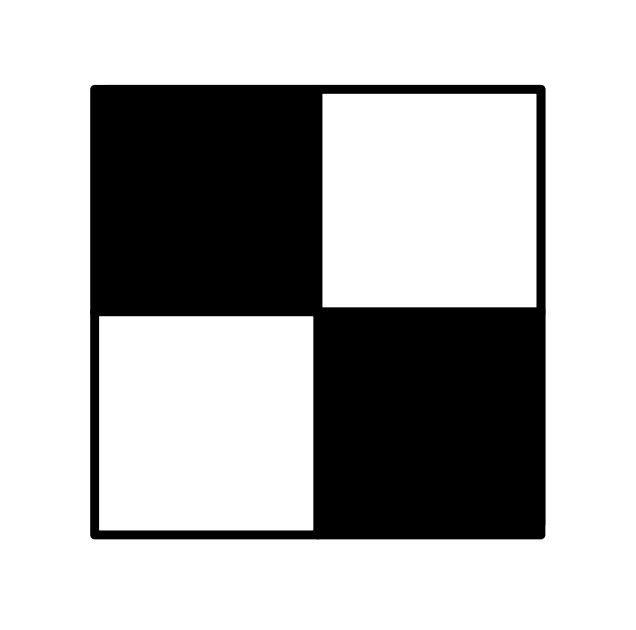
\includegraphics[scale=1]{eckmanhilton2.png}
\end{center}

\begin{center}
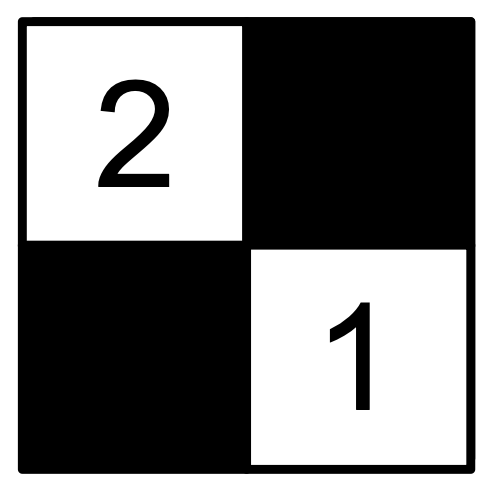
\includegraphics[scale=1]{r1.png}
\end{center}

\begin{center}
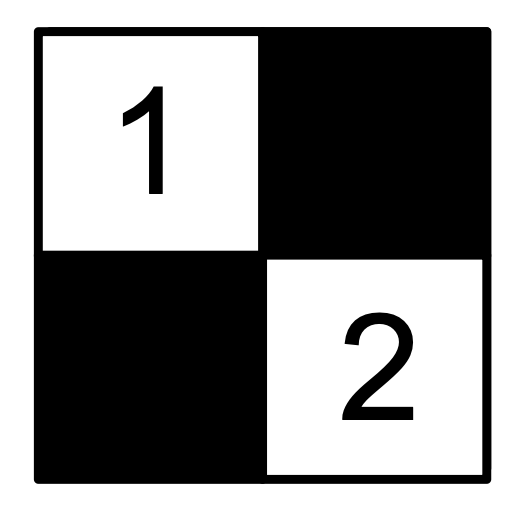
\includegraphics[scale=1]{r2.png}
\end{center}

\begin{center}
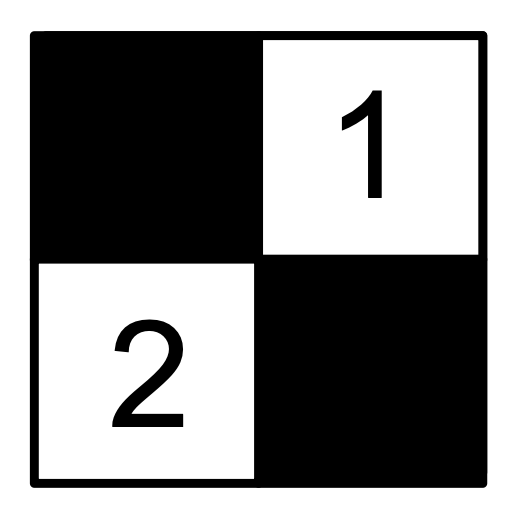
\includegraphics[scale=1]{r3.png}
\end{center}

\begin{center}
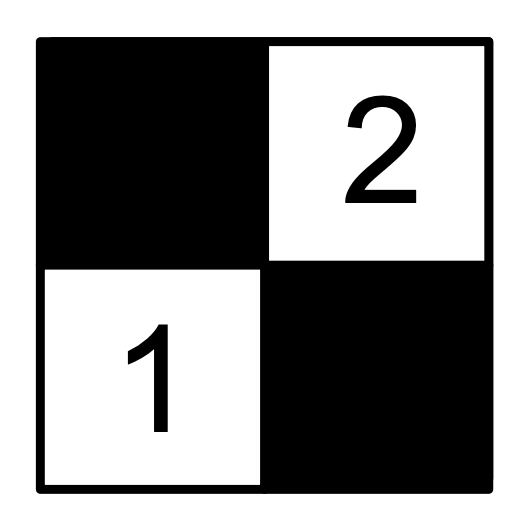
\includegraphics[scale=1]{r4.png}
\end{center}



\begin{center}
OperadicGroup 2 ∞-Grpd₋₁
\end{center}

\begin{center}

\end{center}

\iffalse
B¹.obj (M × N) ⭢ (B¹.obj M) × (B¹.obj N)
\fi

\section{B¹ and Bⁿ}

\begin{definition}
B¹ 
\end{definition}

\begin{definition}
Bⁿ is B¹ • Bⁿ⁻¹.
\end{definition}

\subsection{The Postnikov Tower}

Here I would like to construct the Postnikov tower from a different perspective, using B¹.\\

\subsection{The Whitehead Tower}

Here I would like to construct the Whitehead tower from a different perspective, using B¹.\\



\section{Chain Complexes}




\section{Realization of Chain Complexes}




\section{Tensor Product of Chain Complexes}



\newpage
\chapter{Tensor Product}

\begin{enumerate}
\item \iffalse https://leanprover-community.github.io/mathlib4_docs/Mathlib/LinearAlgebra/TensorProduct/Basic.html#TensorProduct \fi
\end{enumerate}


\newpage
\chapter{Tensor Product of ∞-Spaces}

\iffalse
∧\_(∞-Spc)
\fi

∞-Grpd₋₁ with smash product forms an operadic commutative monoid, but not a monoidal category.\\


\newpage
\chapter{Set₋₁ ⇄ AbelianGroup}


{
\footnotesize
\begin{center}
\begin{tabular}{||l | l ||} 
 \hline
 Construction & Description \\
 \hline
??? : InternalAbelianGroup Set₋₁ ≅ AbelianGroup : ???  & The ??? theorem \\
\hline
??? : Set₋₁ ⇄ AbelianGroup : ??? & The ??? adjunction \\
 \hline
\end{tabular}
\end{center}
}

Abelian groups are internal groups in internal groups in sets.\\


In forming the free group on a set, based sets intermediate the construction.\\



\newpage
\chapter{∞-Grpd₋₁ ⇄ ∞-Space}

In this section, we construct a 
{
\footnotesize
\begin{center}
\begin{tabular}{||l | l ||} 
 \hline
 Construction & Description \\
 \hline
 ??? : InternalAbelianGroup Set₋₁ ≅ AbelianGroup : ???  & The ??? theorem \\
\hline
 ??? : ∞-Grpd₋₁ ⇄ ∞-Space : ??? & The ??? adjunction \\
 \hline
\end{tabular}
\end{center}
}


\begin{enumerate}
\item πₙ of an ∞-space arising from an ∞-groupoid
\item Hₙ of an 
\item Dold-Thom theorem
\item \iffalse https://leanprover.zulipchat.com/#narrow/stream/116395-maths/topic/homology \fi
\item B is iterable on this
\item Chn ... 
\item μ : Chn × Chn ⭢ Chn
\end{enumerate}


S\_(???) in general...


\iffalse
In forming the free ∞-space on an ∞-groupoid, based ∞-groupoids intermediate the construction.
\fi

\iffalse
{
\footnotesize
\begin{center}
\begin{tabular}{||l || l || l ||} 
 \hline
 & \multicolumn{2}{||c||}{\texttt{Eight Free Constructions in Algebra}} \\
 \hline
 \hline 
 & \multicolumn{2}{||c||}{\texttt{Cartesian}} \\
 \hline
  & \texttt{Strict} & \texttt{Lax}   \\
 \hline
 \texttt{Unitial}  & ??? : Map ??? ⇄ InternalAbelianGroup (Map ???) : ??? & ??? : Map ??? ⇄ (OperadicAbelianGroup (Map ???)) : ???  \\
 \hline
 \texttt{Actional} & ??? : ??? ⇄ InternalAbelianGroupAction ??? : ??? & ??? : ??? ⇄ OperadicAbelianGroupAction ??? : ??? \\
 \hline
 \hline
  & \multicolumn{2}{||c||}{\texttt{Tensorial}} \\
 \hline
  & \texttt{Strict} & \texttt{Lax}   \\
 \hline
 \texttt{Unitial}  & ??? : ∞-Grpd₋₁ ⇄ InternalAbelianGroup : ???  &  ??? : ??? ⇄ OperadicAbelianGroup ∞-Grpd₋₁ : ???  \\
 \hline
 \texttt{Actional} & ??? : ??? ⇄ InternalAbelianGroupAction ???  : ???  &  ??? : ??? ⇄ OperadicAbelianGroupAction ??? : ??? \\
 \hline
\end{tabular}
\end{center}
}











  & \multicolumn{2}{||c||}{\texttt{Tensorial}} \\
 \hline
  & \texttt{Strict} & \texttt{Lax}   \\
 \hline
 \texttt{Unitial}  & ??? : ∞-Grpd₋₁ ⇄ InternalAbelianGroup  : ???  &  ??? : ??? ⇄ OperadicAbelianGroup ∞-Grpd₋₁ : ???  \\
 \hline
 \texttt{Actional} & ??? : ??? ⇄ InternalAbelianGroupAction ???  : ???  &  ??? : ??? ⇄ OperadicAbelianGroupAction ??? : ??? \\
 \hline














 \iffalse
  \hline
    \texttt{InternalAbelianGroup Ch² AbelianGroup}  & \texttt{InternalAbelianGrouAction Ch² AbelianGroup} & \texttt{OperadicAbelianGroup ∞-Ch² ∞-Space} & \texttt{OperadicAbelianGroupAction ∞-Ch² ∞-Space} \\ 
{
\footnotesize
\begin{center}
\begin{tabular}{||l || l || l || l ||} 
 \hline
  \multicolumn{4}{||c||}{\texttt{??? Structures}} \\
 \hline
 \multicolumn{2}{||c||}{\texttt{Strict}}  &  \multicolumn{2}{||c||}{\texttt{Lax}} \\
 \hline
 \texttt{Unitial} &  \texttt{Actional}  &  \texttt{Unitial} &  \texttt{Actional}\\
 \hline \hline
 \texttt{InternalMonoid AbelianGroup}  & \texttt{InternalMonoidAction AbelianGroup} & \texttt{OperadicMonoid ∞-Space} & \texttt{OperadicMonoidAction ∞-Space} \\ 
 \hline
  \texttt{InternalMonoid Ch AbelianGroup}  & \texttt{InternalMonoidAction Ch AbelianGroup} & \texttt{OperadicMonoid ∞-Ch ∞-Space} & \texttt{OperadicMonoidAction ∞-Ch ∞-Space} \\ 
  \hline
  \texttt{InternalMonoid Ch² AbelianGroup}  & \texttt{InternalMonoidAction Ch² AbelianGroup} & \texttt{OperadicMonoid ∞-Ch² ∞-Space} & \texttt{OperadicMonoidAction ∞-Ch² ∞-Space} \\ 
  \hline
 \hline
 \texttt{InternalCommutativeMonoid} & \texttt{InternalCommutativeMonoidAction} & \texttt{OperadicCommutativeMonoid} & \texttt{OperadicCommutativeMonoidAction} \\
 \hline
  \texttt{InternalCommutativeMonoid Ch AbelianGroup}  & \texttt{InternalCommutativeMonoidAction Ch AbelianGroup} & \texttt{OperadicCommutativeMonoid ∞-Ch ∞-Space} & \texttt{OperadicMonoidAction ∞-Ch ∞-Space} \\ 
  \hline
  \texttt{InternalCommutativeMonoid Ch² AbelianGroup}  & \texttt{InternalCommutativeMonoidAction Ch² AbelianGroup} & \texttt{OperadicCommutativeMonoid ∞-Ch² ∞-Space} & \texttt{OperadicCommutativeMonoidAction ∞-Ch² ∞-Space} \\ 
  \hline
    \texttt{InternalAbelianGroup Ch² AbelianGroup}  & \texttt{InternalAbelianGrouAction Ch² AbelianGroup} & \texttt{OperadicAbelianGroup ∞-Ch² ∞-Space} & \texttt{OperadicAbelianGroupAction ∞-Ch² ∞-Space} \\ 
 \hline
\end{tabular}
\end{center}
}
\fi


\fi



\part{RINGS, COMMUTATIVE RINGS, A${}^{\infty}$-RINGS, AND E${}^{\infty}$-RINGS}

In this second section, I consider four constructions for monoidal categories which have occured less generally elsewhere for cartesian categories: internal monoids, internal commutative monoids, algebras for $A{}^{\infty}$-operads, and algebras for $E{}^{\infty}$-operads. The main difference with the structures featured previously is that these structures concern an operation which is more general than product, but less general than pullback. Four of the sixteen structures formed in the repository concerning the Whitehead theorem can re-create the rest, are not instances of the structures here. Meanwhile, the four structures defined here will be constructed using Mathlib 4's monoidal categories and symmetric monoidal categories. Tensor product of abelian groups and smash product of ∞-spaces, coincide with the previous structures in the case where the monoidal operation is product (see Fox's theorem).\\

To reflect the use of monoidal categories as opposed to categories (in which the cartesian monoidal structure can be recovered from the structure as a seven entry with the addition of a single Lean universe), I use different names for the constructions:

{
\footnotesize
\begin{center}
\begin{tabular}{||l || l || l || l ||} 
 \hline
  \multicolumn{4}{||c||}{\texttt{Categories of Internal Objects}} \\
 \hline
 \multicolumn{2}{||c||}{\texttt{Strict}}  &  \multicolumn{2}{||c||}{\texttt{Lax}} \\
 \hline \hline
 \texttt{Unitial} &  \texttt{Actional}  &  \texttt{Unitial} &  \texttt{Actional}\\
 \hline 
 \texttt{MonoidObjects : ??? → ???}  & \texttt{MonoidActionObjects : ??? → ???} & A${}^{\infty}$-Monoid ∞-Space & A${}^{\infty}$-MonoidAction ∞-Space \\ 
 \hline
 \texttt{CommutativeMonoidObjects : ??? → ??? } & \texttt{CommutativeMonoidActionObjects : ??? → ???} & E${}^{\infty}$-Monoid ∞-Space & E${}^{\infty}$-MonoidAction ∞-Space \\
 \hline
\end{tabular}
\end{center}
}

\iffalse
{
\footnotesize
\begin{center}
\begin{tabular}{||l || l || l || l ||} 
 \hline
  \multicolumn{4}{||c||}{\texttt{Eckman-Hilton ???}} \\
 \hline
 \multicolumn{2}{||c||}{\texttt{Strict}}  &  \multicolumn{2}{||c||}{\texttt{Lax}} \\
 \hline
 \texttt{Unitial} &  \texttt{Actional}  &  \texttt{Unitial} &  \texttt{Actional}\\
 \hline \hline
 \texttt{MonoidObjects AbelianGroup}  & \texttt{MonoidActionObjects AbelianGroup} & \texttt{A${}^{\infty}$-Monoid ∞-Space} & \texttt{A${}^{\infty}$-MonoidAction ∞-Space} \\ 
 \hline
  \texttt{MonoidObjects (Chn AbelianGroup)}  & \texttt{{MonoidActionObjects (Chn AbelianGroup)} & \texttt{A${}^{\infty}$-Monoid (∞-Chn ∞-Space)} & \texttt{A${}^{\infty}$-MonoidAction (∞-Chn ∞-Space)} \\ 
 \hline
 \hline
 \texttt{CommutativeMonoidObjects} & \texttt{CommutativeMonoidActionObjects} & \texttt{OperadicCommutativeMonoid} & \texttt{OperadicCommutativeMonoidAction} \\
 \hline
  \texttt{CommutativeMonoidObjects Chn AbelianGroup}  & \texttt{InternalCommutativeMonoidAction (Chn AbelianGroup)} & \texttt{OperadicCommutativeMonoid (∞-Chn ∞-Space)} & \texttt{OperadicMonoidAction (∞-Chn ∞-Space)} \\
 \hline
\end{tabular}
\end{center}
}
\fi


\newpage
\chapter{Rings and Commutative Rings}

Rings and DGAs

Commutative rings and CDGAs

\begin{enumerate}
\item \href{https://leanprover.zulipchat.com/#narrow/stream/287929-mathlib4/topic/Category.20of.20Commutative.20Algebras}{A thread on} creating the six-entry category of commutative algebras.
\item In this section we use slightly different internal structures than the internal monoid in the last section; these internal monoids are defined in a monoidal category and the others are defined for product only. As such we may like to re-examine those structures, or alternatively to keep separate definitions.
\item What's more clear is that the ∞-analogous are more difficult to reconcile with the choices made for the first sixteen structures and the four doubled structures (see the section on the Eckman-Hilton argument)
\end{enumerate}



\newpage
\chapter{A${}^{\infty}$-Rings and E${}^{\infty}$-Rings}

\iffalse
A${}^{\infty}$-Rings and DG A${}^{\infty}$-Rings
E${}^{\infty}$-Rings and DG E${}^{\infty}$-Rings

Commutative rings and CDGAs
\fi


make sure to include Alg

\iffalse
Besides that my ∞-spaces are different, I would like to make my Ainfinity and Einfinity objects as similar as possible.
\fi

make sure to include ∞-Alg...

\iffalse
- Embedding Ringᵒᵖ into ∞-presheaves in ∞-spaces
\fi

\iffalse
https://leanprover.zulipchat.com/#narrow/stream/116395-maths/topic/Ext.20and.20Tor
\fi

\iffalse
https://leanprover.zulipchat.com/#narrow/stream/116395-maths/topic/CDGAs
\fi

\iffalse
https://leanprover.zulipchat.com/#narrow/stream/116395-maths/topic/Tensor.20products.20of.20graded.20objects.20.2F.20chain.20complexes
\fi

\begin{enumerate}
\item What's more clear is that the ∞-analogous are more difficult to reconcile with the choices made for the first sixteen structures and the four doubled structures (see the section on the Eckman-Hilton argument).
\end{enumerate}

\iffalse
C ⊗??? ⭢ ??? ⭢ ??? ⭢ 0
\fi



\newpage
\chapter{Modules over Rings and Commutative Rings}




\newpage
\chapter{A${}^{\infty}$-Modules and E${}^{\infty}$-Modules}





\part{DERIVATIONS AND CONNECTIONS}

In this section, I define four more structures:

{
\footnotesize
\begin{center}
\begin{tabular}{||l || l || l ||} 
 \hline
 & \multicolumn{2}{||c||}{\texttt{Four Definitions}} \\
 \hline
 & \texttt{Strict} & \texttt{Lax} \\
 \hline
 \texttt{Unitial}  & Derivation & ∞-Derivation \\
 \hline
 \texttt{Actional} & Connection & ∞-Connection \\
 \hline
\end{tabular}
\end{center}
}

I also construct four adjunctions which feature the internal abelian group structure:

{
\footnotesize
\begin{center}
\begin{tabular}{||l || l || l ||} 
 \hline
 & \multicolumn{2}{||c||}{\texttt{Four Free Constructions in Algebra}} \\
 \hline
 \hline
  & \texttt{Strict} & \texttt{Lax}   \\
 \hline
 \texttt{Unitial}  & ??? : Map ??? ⇄ InternalAbelianGroup (Map ???) : ??? & ??? : Map ??? ⇄ (OperadicAbelianGroup (Map ???)) : ???  \\
 \hline
 \texttt{Actional} & ??? : ??? ⇄ InternalAbelianGroupAction ??? : ??? & ??? : ??? ⇄ OperadicAbelianGroupAction ??? : ??? \\
 \hline
\end{tabular}
\end{center}
}

In this second part, I define eight adjunctions associated to the algebraic structures defined in the last section.\\



\newpage
\chapter{Lie Algebras}

\begin{definition}[Lie Algebra] Let $A$ be a (commutative unitial) ring. A Lie-algebra is an $A$-module $M$ such that...
\end{definition}

\begin{definition}[Lie Algebra Map] Let $A$ be a (commutative unitial) ring.
\end{definition}

\begin{enumerate}
\item \href{https://leanprover.zulipchat.com/#narrow/stream/287929-mathlib4/topic/The.20classification.20of.20Lie.20algebras}{A thread on the classification of Lie algebras}.
\end{enumerate}

The Jacobi identity says that the lie-bracket is a self-derivation.\\



\newpage
\chapter{Derivations}

In a blog post \href{https://amathew.wordpress.com/2011/05/14/the-cotangent-complex-i-group-objects-in-categories-of-algebras/}{here},



Let $\texttt{A}$ be a ring and suppose that $\texttt{B : Alg A}$. $\texttt{B.dom}$.\\

\begin{center}
S\_(Mon (Act R))𛲔 : (ComMon R) ⇄ ??? : S\_(Mon (Act R))ॱ
\end{center}

\begin{theorem}the category of internal abelian groups in Mon (Act R) is equivalent to Act R
\end{theorem}

\begin{center}
S\_(Mon (Ch (Act R)))𛲔 : Mon (Ch (Act R)) ⇄ Mod R : S\_(Mon (Ch (Act R)))ॱ
\end{center}


\begin{center}
(Alg A)⁄A ⇄ (Alg A)
\end{center}


\begin{enumerate}
\item I would like to first construct the lie-algebra of derivations using the spectrum \texttt{Ωⁱⁿᶠ.obj X}. It seems related to coalgebra endomorphisms from \texttt{Ωⁱⁿᶠ.obj X} to itself.
\item Lie algebras and Derₖ(A,A)
\end{enumerate}


\newpage
\chapter{L${}^{\infty}$ Algebras}




\newpage
\chapter{∞-Derivations}

\begin{center}
Ω\_()𛲔 : (Eⁱⁿᶠ-Alg A)/A ⇄ Eⁱⁿᶠ-Mod A : Ω\_()ॱ
\end{center}

\begin{center}
Λ\_()𛲔 : Ch (Eⁱⁿᶠ-Alg A) ⇄ Eⁱⁿᶠ-Mod A : Λ\_()ॱ
\end{center}



In this section, I construct: 

\begin{center}
Ωⁱⁿᶠ\_(A) : (E${}^{\infty}$-Alg A)⁄A ⇄ E${}^{\infty}$-Mod A : Λⁱⁿᶠॱ\_(A)
\end{center}

And I also define the concept of an ∞-derivation.\\

This adjunction factors like so:

\begin{center}
Ωⁱⁿᶠ\_(A) : (E${}^{\infty}$-Alg A)⁄A ⇄ ??? ⇄ E${}^{\infty}$-Mod A : Λⁱⁿᶠॱ\_(A)
\end{center}


The more typical concept of a free abelian group .\\


Given an $E^{\infty}$-algebra...., we can form an \\
\iffalse
https://golem.ph.utexas.edu/category/2011/05/an_operadic_introduction_to_en.html
\fi

\iffalse
https://arxiv.org/pdf/1106.1791.pdf
\fi


\newpage
\chapter{Tensor Product of Lie-Algebras}




\newpage
\chapter{Tensor Product of L${}^{\infty}$-Algebras}




\newpage
\chapter{Connections}

s instead of ω and λ

\iffalse
\begin{center}
ω\_()𛲔 : (Eⁱⁿᶠ-Mod A) ⇄ Eⁱⁿᶠ-Mod A : ω\_()ॱ
\end{center}

\begin{center}
λ\_()𛲔 : Ch (Eⁱⁿᶠ-Mod A) ⇄ Eⁱⁿᶠ-Mod A : λ\_()ॱ
\end{center}
\fi

The set of connections forms an affine space. One can then define:

\iffalse
\begin{enumerate}
... ⭢ Ω¹(...)
\end{enumerate}
\fi



\begin{enumerate}
\item Free abelian group action.
\end{enumerate}

\iffalse
https://amathew.wordpress.com/2011/05/14/the-cotangent-complex-i-group-objects-in-categories-of-algebras/
\fi

\iffalse
https://en.wikipedia.org/wiki/Connection_(vector_bundle)
\fi

A connection on a vector bundle can be understood as an element of:

\begin{enumerate}
\item the free graded module given a connection
\item Ω⁰(X) ⊗ V ⭢ Ω¹(X) ⊗ V such that (∇ X) f ⊗ x = (df) ⊗ x + f((∇ X) (1 ⊗ x))
\item Ω¹([V,V])
\end{enumerate}

This can be understood in terms of the theorem that End${}_{A}$(V ⊗ A) is isomorphic to End${}_{k}$(V) ⊗ A for a free A-module V and certain condition on the k-algebra $A$, where we here take A to be Ωॱ(X).\\

We can understand the first in terms of the Ω⁰(X)-module Ωⁿ(X) ⊗ [V,V] ⭢ Ωⁿ⁺¹(X) ⊗ [V,V] in which we extend ∇ to feature a the rule of (df) ⊗ x + (-1)ⁱʲ * f((∇ X) (1 ⊗ x)), and write $d_{∇}$ for this, but it doesn't form a chain complex. Instead, we obtain an element of Ω²([V,V]) from $d_{∇} d_{∇} x$ for any section $x$ of $V$. Defining $F_{∇}$ to be dA - A ∧ A, wedge with $F_{∇}$ is the same as $d_{∇} d_{∇}$.\\

\iffalse
If A and B are matrices close enough to 1, then we can unambiguously take their logarithm after pulling back to a square whose diagonal has a 2-norm of 1 or less.\\
\fi

\iffalse
https://mathoverflow.net/questions/455423/obstructions-to-the-existence-of-a-flat-connection-on-a-vector-bundle
\fi


\newpage
\chapter{∞-Connections}

Connections are elements of the free abelian group action on an A-algebra over A, and ∞-connections are ...\\

\iffalse
https://en.wikipedia.org/wiki/Connection_(vector_bundle)
\fi

\begin{enumerate}
\item I would like to first construct the lie-algebra representation of flat connections using the spectrum \texttt{ωⁱⁿᶠ.obj X).obj V}.
\item \iffalse https://en.wikipedia.org/wiki/Connection_(vector_bundle)\fi
\item Lie algebra representations and ...
\item 
\item 
\item \iffalse https://en.wikipedia.org/wiki/Connection_(vector_bundle)\fi
\item Somehow connections are the dual of the free abelian group action
\end{enumerate}

\iffalse We can define differentiable and connective functionals in this context as well. \fi

\iffalse
https://en.wikipedia.org/wiki/Connection_form
\fi

\iffalse
https://amathew.wordpress.com/2011/05/14/the-cotangent-complex-i-group-objects-in-categories-of-algebras/
\fi

\iffalse
I loaded them up onto degree negative one.
\fi

Some goals:
\begin{enumerate}
\item 
\end{enumerate}

\begin{enumerate}
\item smooth (etale locally ???)
\item analytic (etale locally ???)
\item [ℂP¹,ℂP¹] ≅ ℂ(x)
\item Our ℝ is ∂.obj ℤ regarded as an object in [γ⃗,∞\_(∞-Grpd)]
\item B.obj det : B.obj U(n) ⭢ B.obj U(1)
\item Which E${}_{\infty}$ Space have a Chern class?
\end{enumerate}

Cohomology with coefficients in $\texttt{[-,Bℂˣ]}$ plays a .\\

\iffalse
https://www.universiteitleiden.nl/binaries/content/assets/science/mi/scripties/bachbecker.pdf
\fi

\begin{enumerate}
\item \iffalse https://en.wikipedia.org/wiki/Connection_(vector_bundle) \fi
\item d2 is wedge with (representable...)
\end{enumerate}

Given an $E^{\infty}$-algebra...., we can form an \\


\iffalse
https://en.wikipedia.org/wiki/Connection_(vector_bundle)
\fi


\newpage
\chapter{Tensor Product of Lie-Algebra Representations}




\newpage
\chapter{L${}^{\infty}$-Algebra Representations}




\newpage
\chapter{Bibliography}

\begin{enumerate}
\item Samuel Eilenberg and Saunders Mac Lane, "On the Groups H(π, n). I", Annals of Mathematics, Second Series, Vol. 58, No. 1 (Jul., 1953), pp. 55-106.
\item Samuel Eilenberg and Saunders Mac Lane, "On the Groups H(π, n). II", Annals of Mathematics, Second Series, Vol. 60, No. 1 (Jul., 1954), pp. 49-139.
\item Saunders Mac Lane, "On the Homology Theory of Eilenberg-Mac Lane", Proceedings of the National Academy of Sciences of the United States of America, Vol. 35, No. 11 (Nov. 15, 1949), pp. 657-663.
\item Eilenberg, S., \& MacLane, S. (1945). Relations Between Homology and Homotopy Groups of Spaces. Proceedings of the National Academy of Sciences of the United States of America, 31(2), 83–87. 
\item Stasheff, J. (Year). L-infinity and A-infinity structures. Higher Structures, Volume(Issue), Page numbers. Retrieved from [URL]
\end{enumerate}

Further reading:

\begin{enumerate}
\item \href{https://www.math.upenn.edu/events/seminars/deformation-theory-seminar?field_date_value%5Bvalue%5D%5Byear%5D=}{A seminar on deformation theory at the university of Pennsylvania}
\item \href{https://ncatlab.org/nlab/show/Gamma-space}{The nlab article on ∞-spaces}
\item \href{https://amathew.wordpress.com/2012/09/16/segals-infinite-loop-space-machine/}{A blog post of Akhil Matthew explaining how Bⁿ X ≅ Ω Bⁿ⁺¹ X for an ∞-space X and n ≥ 2}
\item \href{https://ncatlab.org/nlab/show/Eckmann-Hilton+argument#:~:text=In%20its%20original%20form%2C%20the,or%20Groups%20is%20necessarily%20commutative.}{The n-lab article on the Eckman-Hilton argument}
\item \href{http://www.math.uchicago.edu/~may/PAPERS/mayi.pdf}{Operads, Algebras, and Modules}, an exposition of J. P. May.
\item \href{https://www.math.upenn.edu/events/special-seminar-infinity-category-theory-undergraduates}{A 2022 seminar on ∞-categories for undergraduates}. 
\end{enumerate}


\newpage
\ \\
\thispagestyle{empty}

\end{document}



